\documentclass[11pt]{article}
\usepackage{geometry}                % See geometry.pdf to learn the layout options. There are lots.
\geometry{letterpaper}                   % ... or a4paper or a5paper or ... 
%\geometry{landscape}                % Activate for for rotated page geometry
%\usepackage[parfill]{parskip}    % Activate to begin paragraphs with an empty line rather than an indent
\usepackage{graphicx}
\usepackage{amssymb}
\usepackage{amsmath}
\usepackage{epstopdf}
\usepackage{hyperref}
\DeclareGraphicsRule{.tif}{png}{.png}{`convert #1 `dirname #1`/`basename #1 .tif`.png}



\graphicspath{
{/Users/Andy/Cruises_Research/IWISE/Notes/figures/OverturnBiases/}
}

\title{Biases of profiling sampling on overturns - Notes}
\author{Andy Pickering}
%\date{}                                           % Activate to display a given date or no date



\begin{document}
\maketitle

\tableofcontents
\newpage


%~~~~~~~~~~~~~~~~~~~~~~~~~~~~~~~~~~~~~~~~~~~~~~~~~~~~~~
\section{Introduction}
%~~~~~~~~~~~~~~~~~~~~~~~~~~~~~~~~~~~~~~~~~~~~~~~~~~~~~~

The purpose of this analysis is to examine errors in the calculation of overturns and dissipation from profiling instruments due to the time taken to complete a profile. If the background density field is being displaced vertically as it is sampled, estimated overturn sizes could be larger or smaller than the true overturn sizes. We resample high-resolution (in time) data to simulate measurement by a profiling instrument. Several scenarios are studied, including those designed to represent McLane moored profilers (MPs) and shipboard CTDs. 


\section{Questions/Goals}

\begin{itemize}
\item What is the magnitude of the error/bias in overturns computed from a profiling instrument?
\item How does it depend on sampling speed?
\item Can we make a correction based on the background vertical velocity?
\end{itemize}



\section{Approach}

We resample data from T-chains (Nash) deployed during IWISE near N2 on the western ridge. These consisted of temperature loggers approximately every 10m in the lower  1500m, with fast sampling in time (1Hz?). Data is gridded onto a 10m, 2min grid, and these data are taken as the `true' values in the following analysis. We then resample the data to mimic a MP or other instrument profiling up and down at a specified speed. Overturns are computed from both the true and resampled data and compared.


%~~~~~~~~~~~~~~
\subsection{Data and codes}

The main folder for work is \\ \verb+/Users/Andy/Cruises_Research/IWISE/S9/Dissipation/OverturnsBiases/+ .\\ \newline 
Data was processed and gridded by JN already and is in files \verb+all_gridded.mat+ and \verb+all_moorings.mat+.  I started with Jonathan's code \verb+compute_thorpe_jn_error_test.m+ and reproduced his results. This code assumes that every profile in T-chain data is sampled along a slant. But in reality only a small portion of the data is sampled along the depth-time path of the profiler. His results are essentially an average over many different phasings.

\vskip

I resample the Tchains in  \verb+ResampMPnew12Nov.m+ to do a similar analysis with a more realistic sampling profile. The basic outline is:

\begin{enumerate}
\item Generate a depth-time vector of profiler position based on specified range, speed, etc.. 
\item Sample the real data (T-chain) along this path by interpolating to each profiler path.
\item The resampled data then has a smaller number of profiles (as sampled above) with times corresponding to the center of each up/down profile.
\item Compute overturns for the total and resampled data and compare results.
\end{enumerate}

%~~~~~~~~
\subsubsection{Code}
Main script for IWISE Tchain data is: \verb+ResampleProfiler_V2.m+. \newline
A set of generic codes I wrote to make sample paths and resample data along them are in Github repository \verb+/SimProfiler/+, located at : (\url{https://github.com/andypicke/SimProfiler}).	


%~~~~~~~~~~~~~~
\subsection{Notes}

The epsilon that is already in the data files JN sent is different than what I get if I recompute it; I use the recomputed epsilon (see \verb+ComputeOverturnsTchainsReal.m+) for all analysis.



\clearpage
%~~~~~~~~~~~~~~~~~~~~~~~~~~~~~~~~~~~~~~~~~~~~~~~~~~~~~~
\section{Data Overview}
%~~~~~~~~~~~~~~~~~~~~~~~~~~~~~~~~~~~~~~~~~~~~~~~~~~~~~~

See \verb+PlotTchainFields.m+. Epsilon at Tchains 1 and 2 looks like it might be dominated by smaller overturns that aren't well resolved by Tchain. Maybe should just just 3 and 4?


\begin{figure}[htbp]
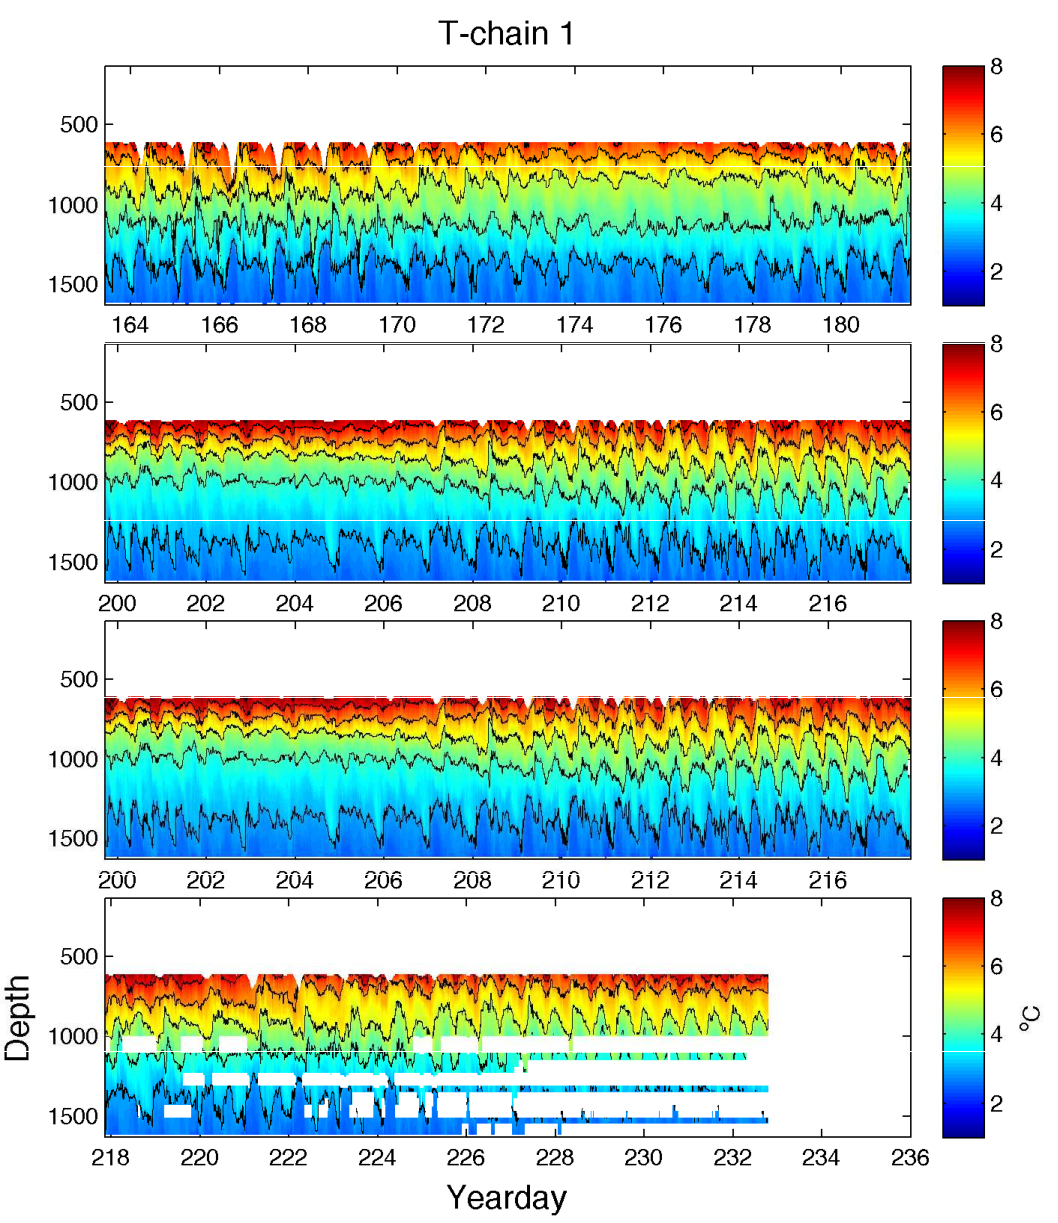
\includegraphics[scale=0.9]{Tchain1_TempOverview.pdf}
\caption{Overview of temperature at Tchain 1.}
\label{}
\end{figure}

\begin{figure}[htbp]
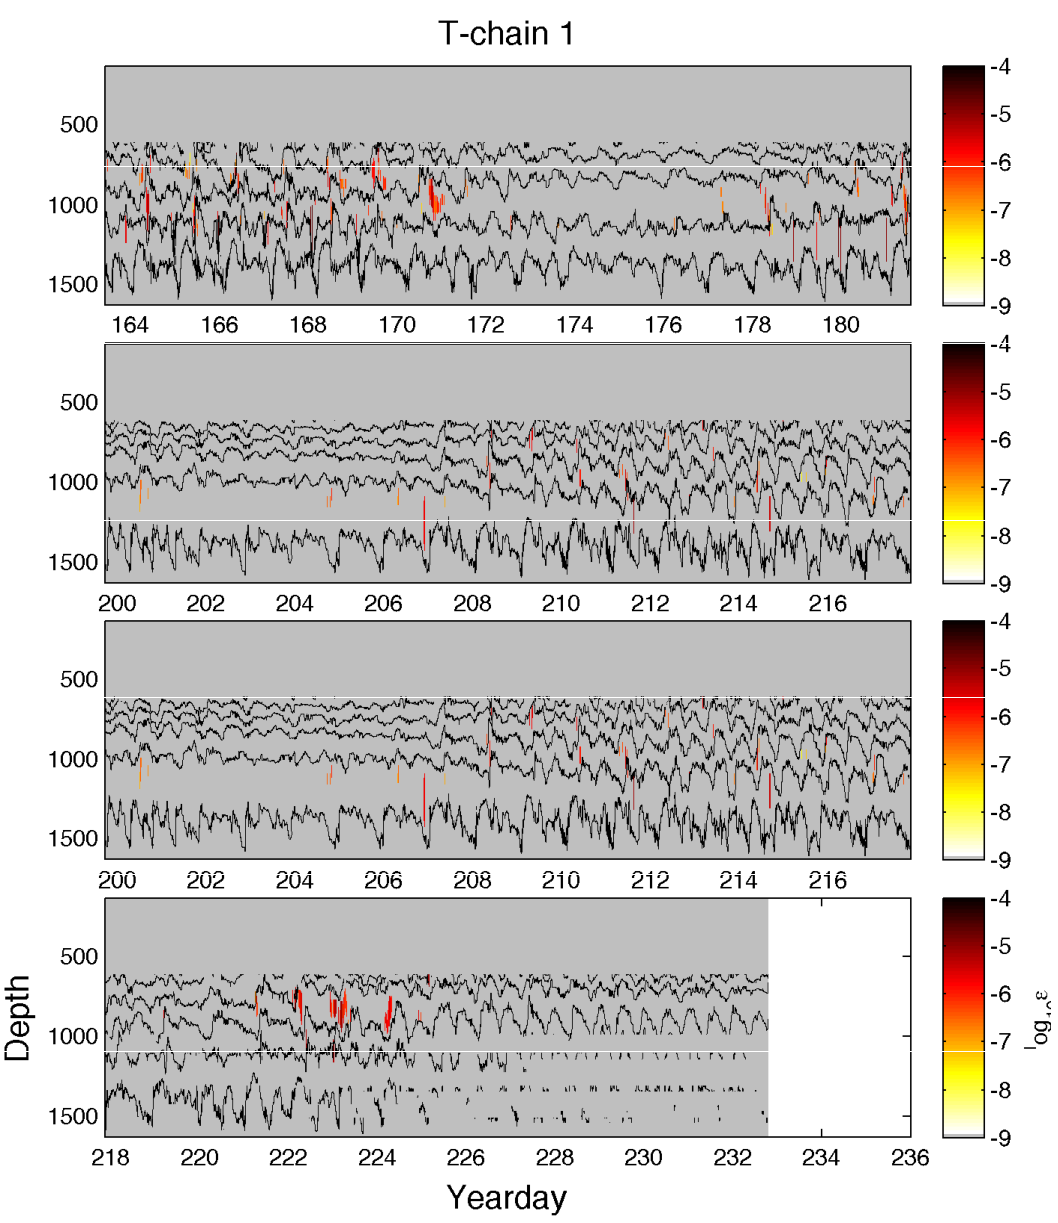
\includegraphics[scale=0.9]{Tchain1_EpsilonOverview.pdf}
\caption{Overview of epsilon (color) and temperature contours at Tchain 1.}
\label{}
\end{figure}


\begin{figure}[htbp]
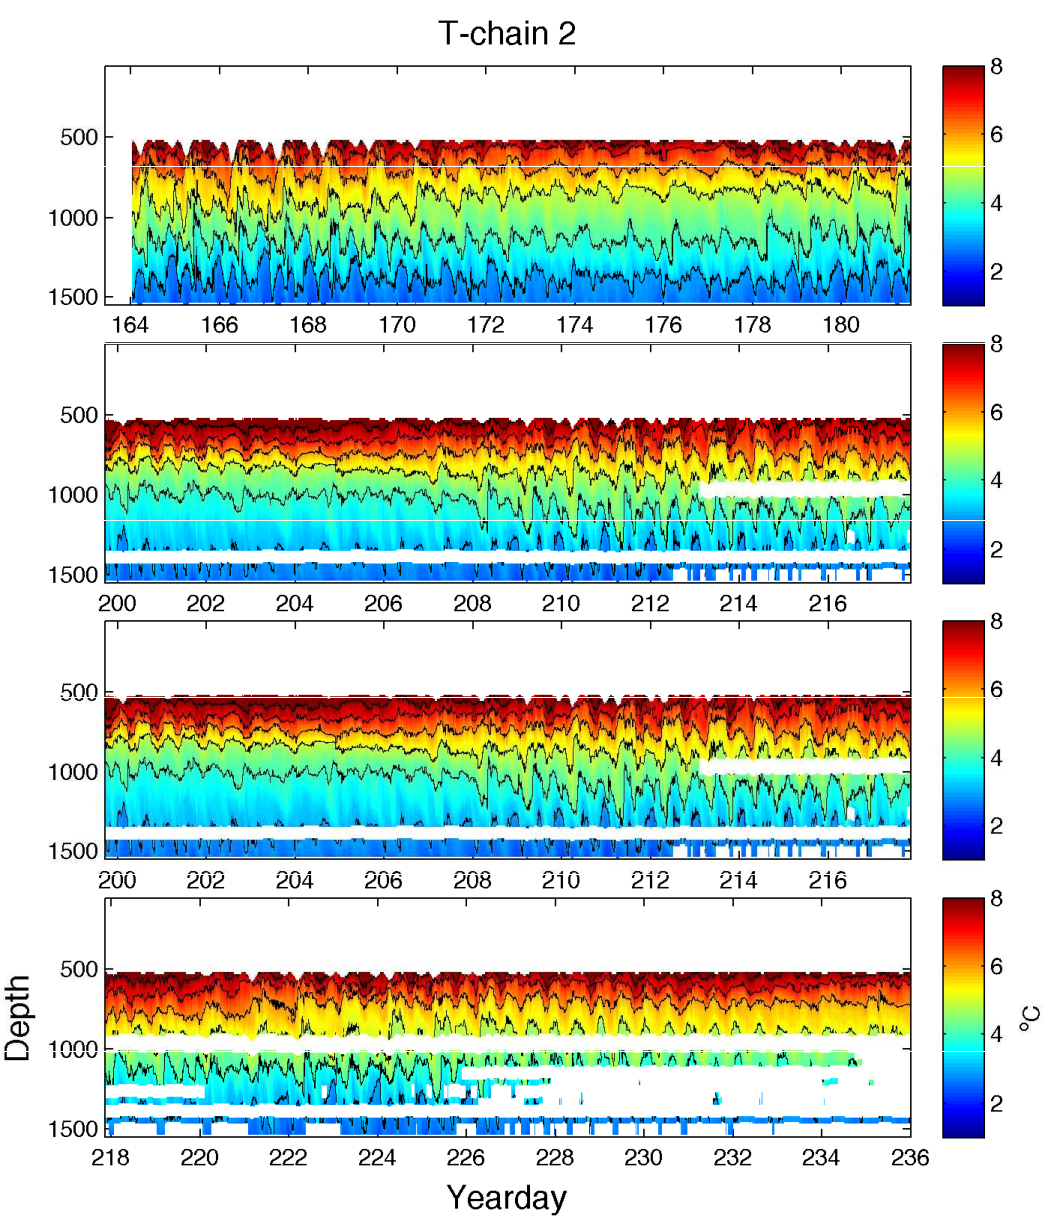
\includegraphics[scale=0.9]{Tchain2_TempOverview.pdf}
\caption{Overview of temperature at Tchain 2.}
\label{}
\end{figure}

\begin{figure}[htbp]
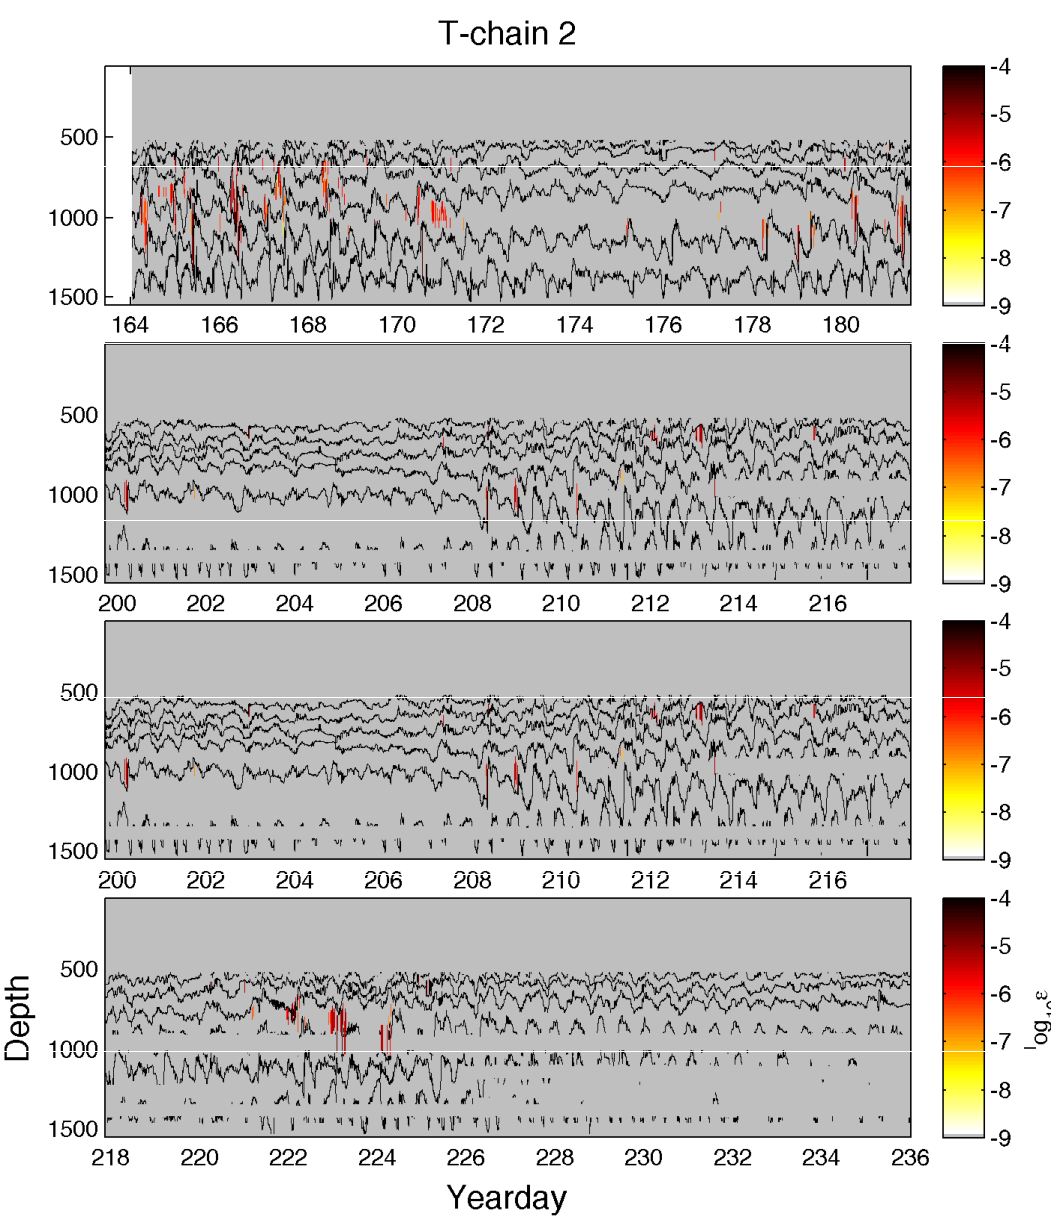
\includegraphics[scale=0.9]{Tchain2_EpsilonOverview.pdf}
\caption{Overview of epsilon (color) and temperature contours at Tchain 2.}
\label{}
\end{figure}


\begin{figure}[htbp]
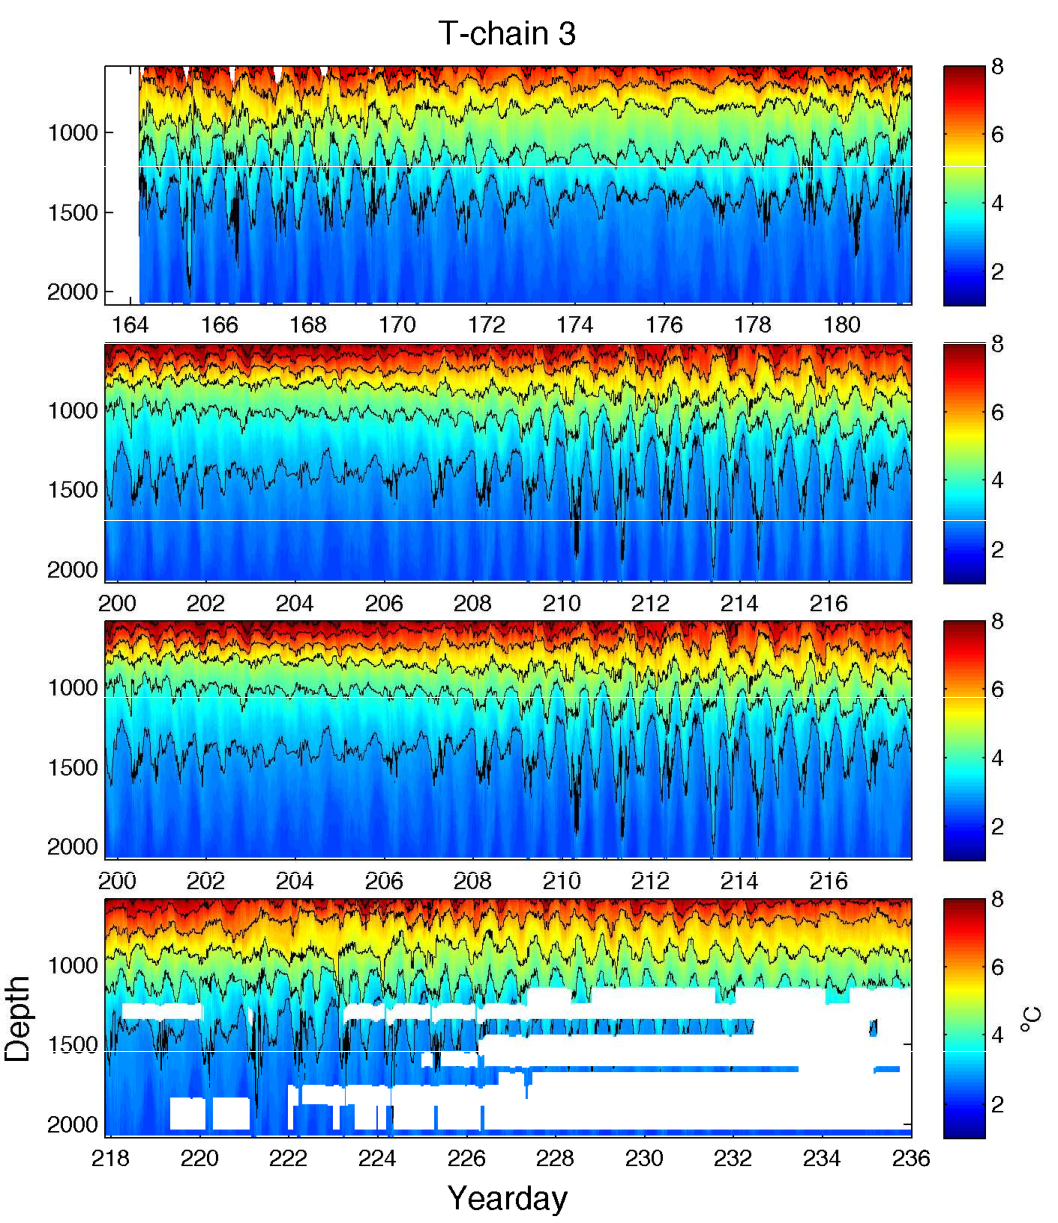
\includegraphics[scale=0.9]{Tchain3_TempOverview.pdf}
\caption{Overview of temperature at Tchain 3.}
\label{}
\end{figure}

\begin{figure}[htbp]
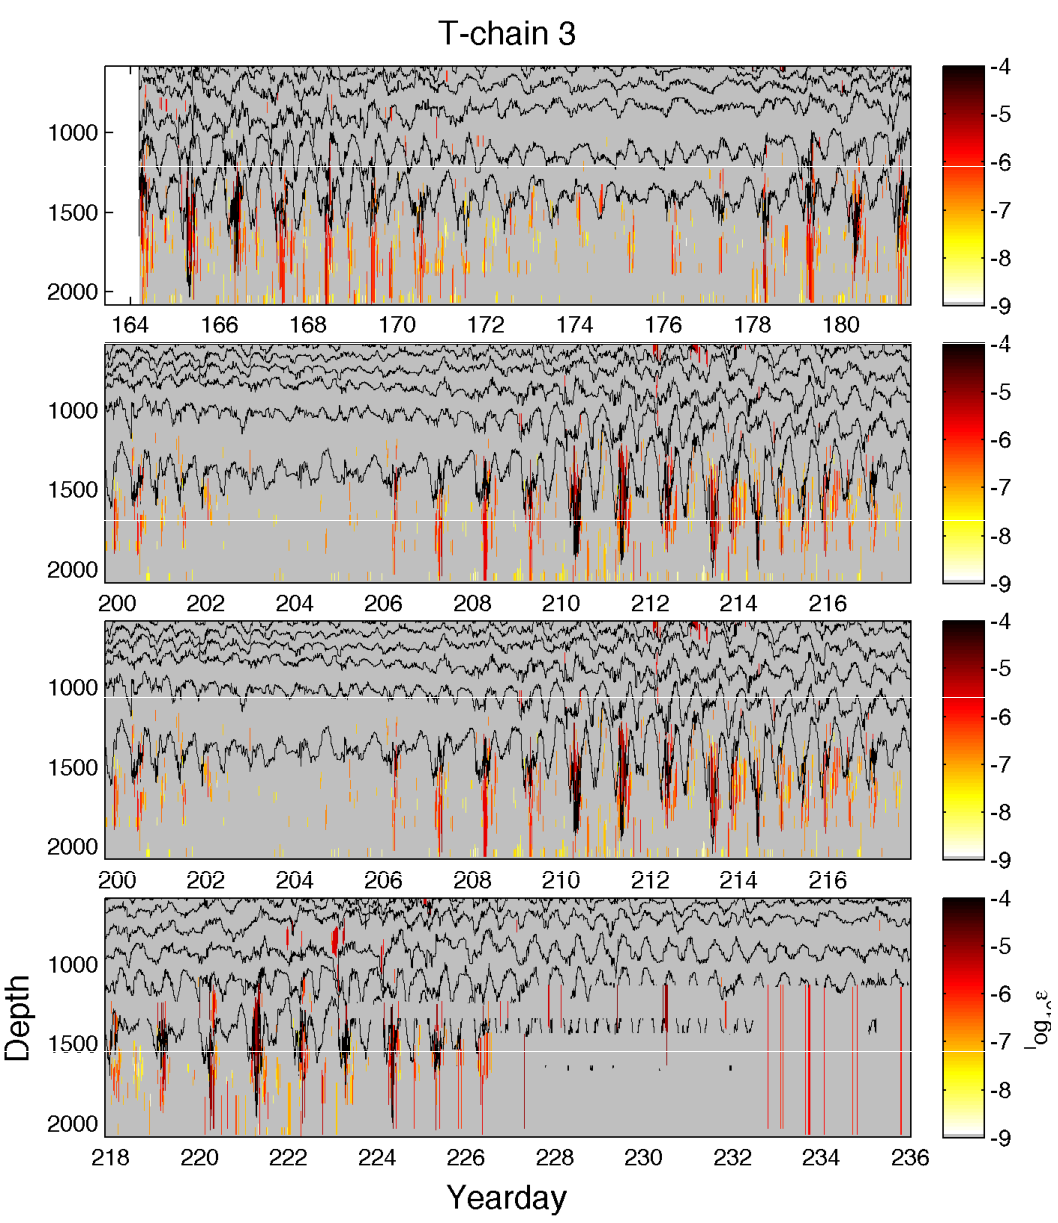
\includegraphics[scale=0.9]{Tchain3_EpsilonOverview.pdf}
\caption{Overview of epsilon (color) and temperature contours at Tchain 3.}
\label{}
\end{figure}


\begin{figure}[htbp]
\includegraphics[scale=0.9]{Tchain4_TempOverview.pdf}
\caption{Overview of temperature at Tchain 4.}
\label{}
\end{figure}

\begin{figure}[htbp]
\includegraphics[scale=0.9]{Tchain4_EpsilonOverview.pdf}
\caption{Overview of epsilon (color) and temperature contours at Tchain 4.}
\label{}
\end{figure}


%
%
%\clearpage
%%~~~~~~~~~~~~~~~~~~~
%\section{Effect of sampling speed}
%
%I ran the resampling for a range of sampling speeds to see the effect on the measured dissipation. I expect the error to decrease with increasing sampling speed.
%\vskip
%See \verb+PlotResampResults12Nov.m+
%
%%%
%\subsection{Tchain 1}
%
%\begin{figure}[htbp]
%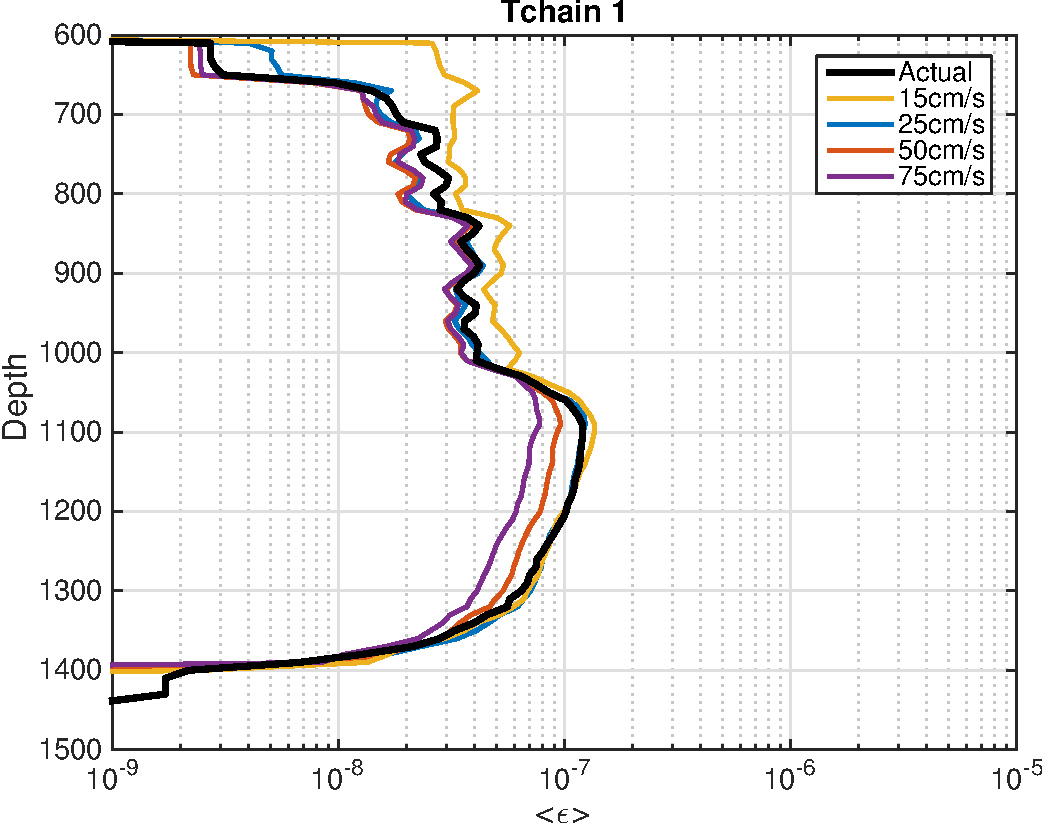
\includegraphics[scale=0.8]{Tchain1_Resamp_EpsvsDepth_DiffSpeeds.pdf}
%\caption{Time-averaged depth profiles of epsilon for different sampling speeds. Black is from raw T chain data, colors are resampled as profiles with different speeds, given in legend.}
%\label{}
%\end{figure}
%
%\begin{figure}[htbp]
%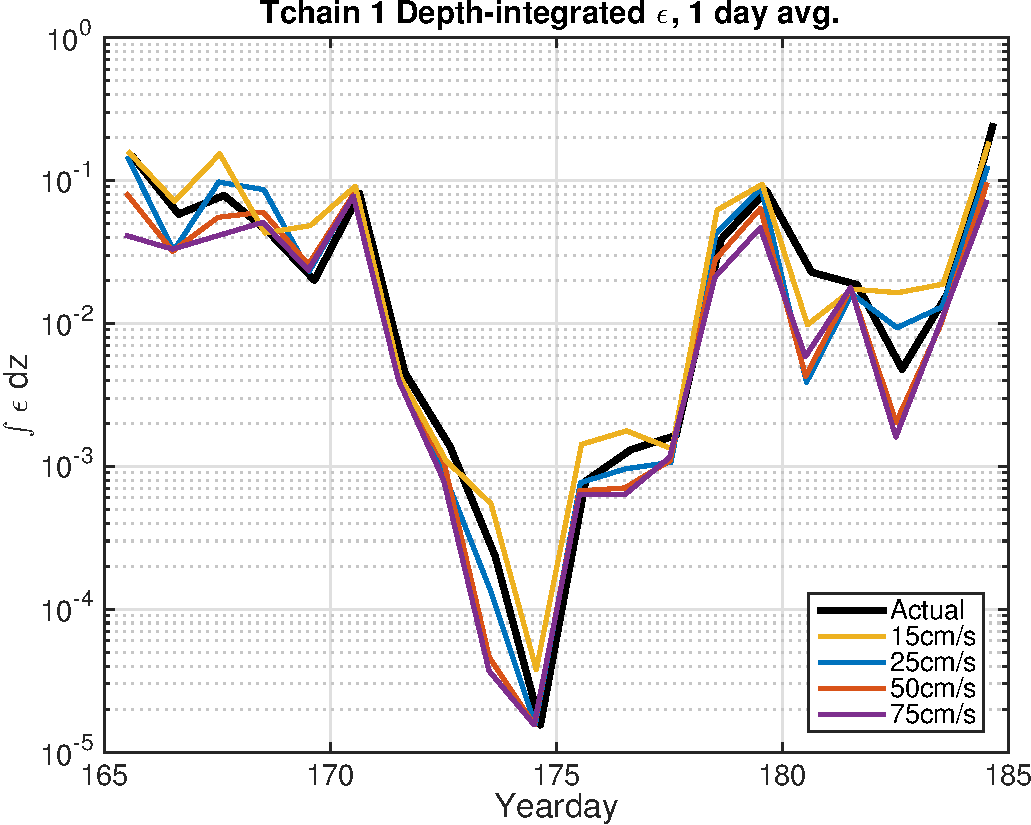
\includegraphics[scale=0.8]{Tchain1_Resamp_IntEpsvsTime_DiffSpeeds.pdf}
%\caption{Timeseries of depth-integrated epsilon for different sampling speeds. Black is from raw T chain data, colors are resampled as profiles with different speeds, given in legend.}
%\label{}
%\end{figure}
%
%
%%%
%\subsection{Tchain 2}
%
%\begin{figure}[htbp]
%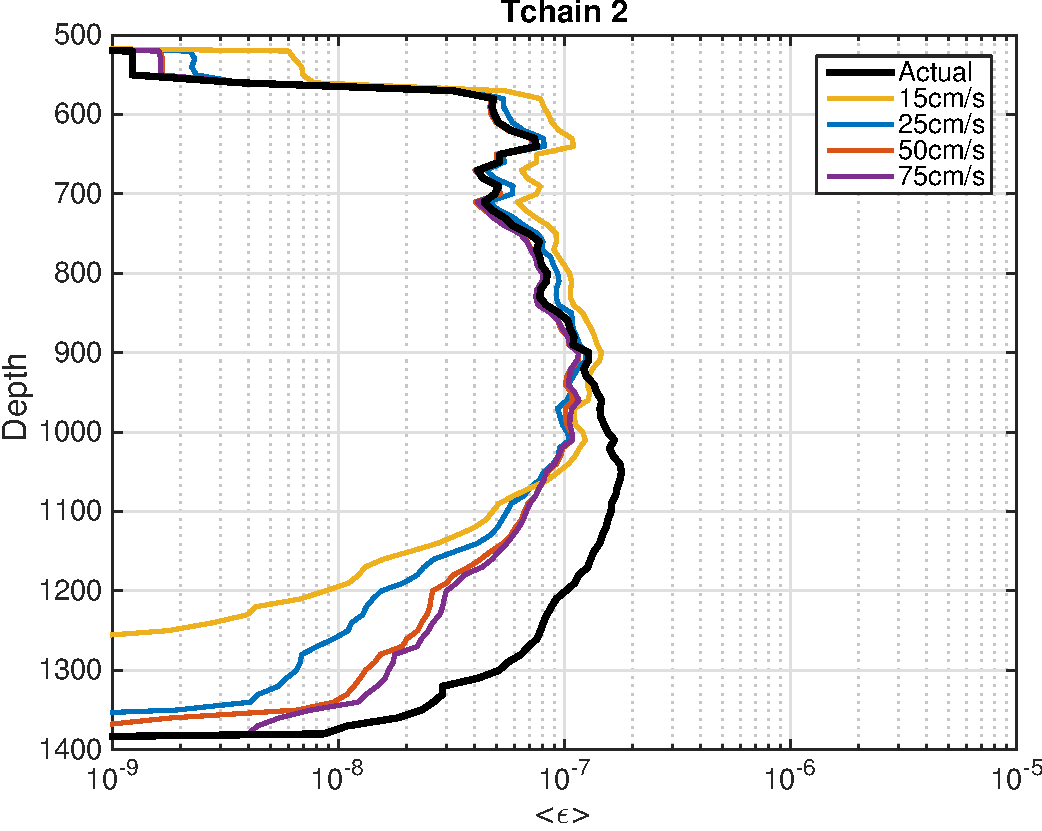
\includegraphics[scale=0.8]{Tchain2_Resamp_EpsvsDepth_DiffSpeeds.pdf}
%\caption{Time-averaged depth profiles of epsilon for different sampling speeds. Black is from raw T chain data, colors are resampled as profiles with different speeds, given in legend.}
%\label{}
%\end{figure}
%
%\begin{figure}[htbp]
%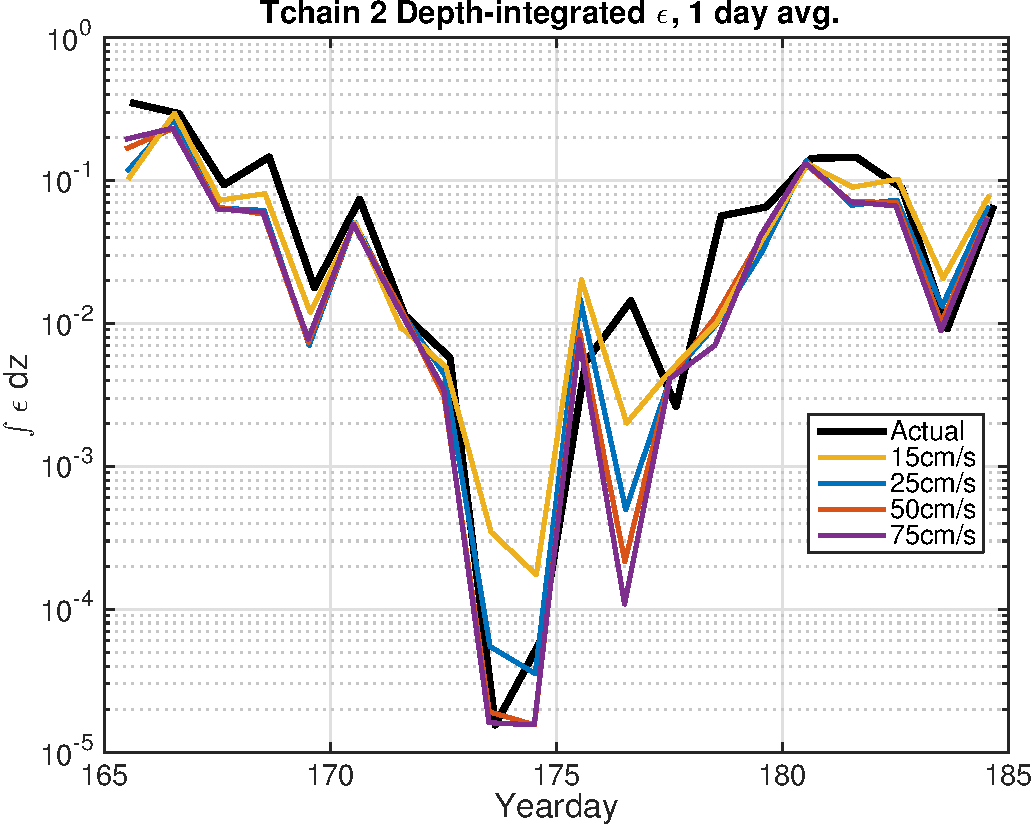
\includegraphics[scale=0.8]{Tchain2_Resamp_IntEpsvsTime_DiffSpeeds.pdf}
%\caption{Timeseries of depth-integrated epsilon for different sampling speeds. Black is from raw T chain data, colors are resampled as profiles with different speeds, given in legend.}
%\label{}
%\end{figure}
%
%
%\clearpage
%%%
%\subsection{Tchain 3}
%\begin{figure}[htbp]
%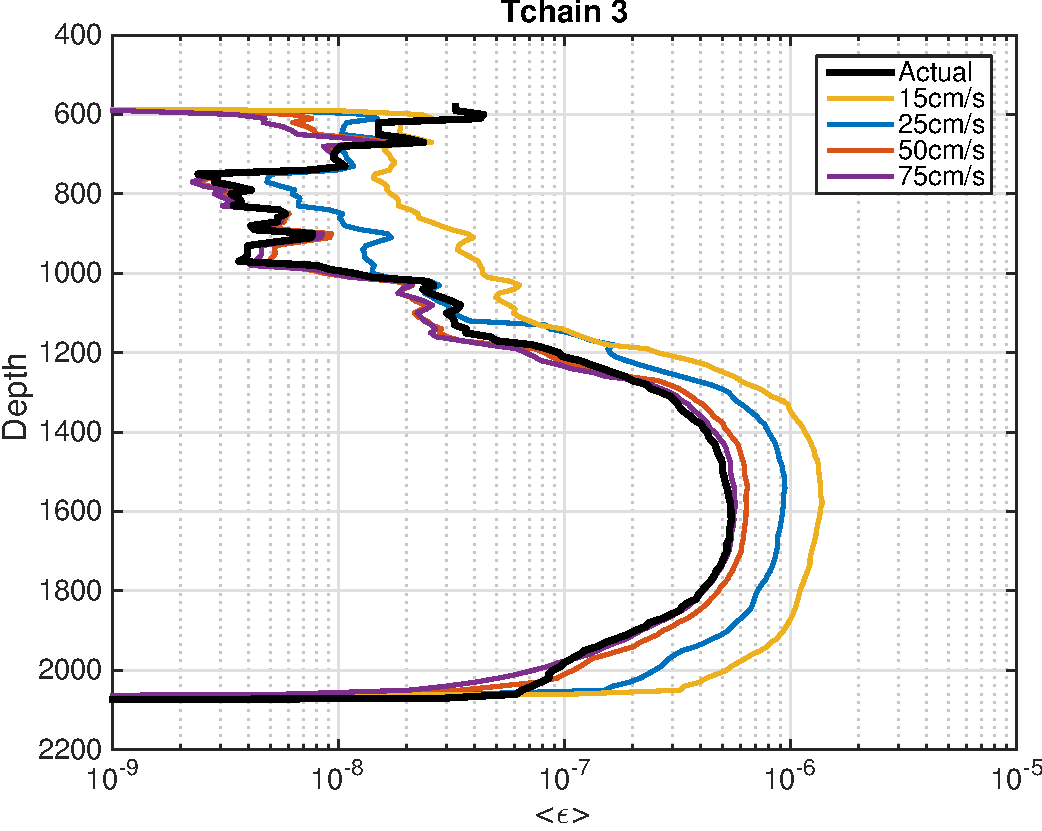
\includegraphics[scale=0.8]{Tchain3_Resamp_EpsvsDepth_DiffSpeeds.pdf}
%\caption{Time-averaged depth profiles of epsilon for different sampling speeds. Black is from raw T chain data, colors are resampled as profiles with different speeds, given in legend.}
%\label{}
%\end{figure}
%
%\begin{figure}[htbp]
%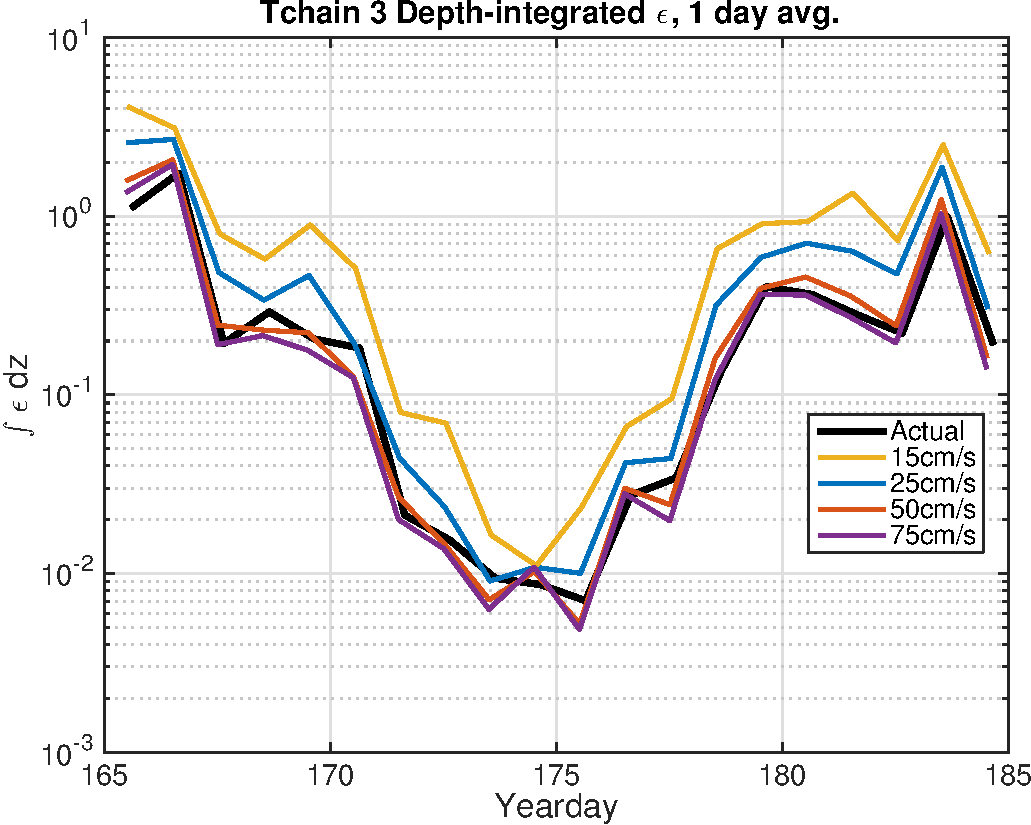
\includegraphics[scale=0.8]{Tchain3_Resamp_IntEpsvsTime_DiffSpeeds.pdf}
%\caption{Timeseries of depth-integrated epsilon for different sampling speeds. Black is from raw T chain data, colors are resampled as profiles with different speeds, given in legend.}
%\label{}
%\end{figure}
%
%\clearpage
%%%
%\subsection{Tchain 4}
%\begin{figure}[htbp]
%\includegraphics[scale=0.8]{Tchain4_Resamp_EpsvsDepth_DiffSpeeds.pdf}
%\caption{Time-averaged depth profiles of epsilon for different sampling speeds. Black is from raw T chain data, colors are resampled as profiles with different speeds, given in legend.}
%\label{}
%\end{figure}
%
%\begin{figure}[htbp]
%\includegraphics[scale=0.8]{Tchain4_Resamp_IntEpsvsTime_DiffSpeeds.pdf}
%\caption{Timeseries of depth-integrated epsilon for different sampling speeds. Black is from raw T chain data, colors are resampled as profiles with different speeds, given in legend.}
%\label{}
%\end{figure}
%


%
%\clearpage
%%~~~~~~~~~~~~~~~~~~~
%\section{Relationship between bias and dissipation magnitude}
%
%It appeared from initial plots that the bias between resampled and true epsilon was proportional to the magnitude of the true epsilon. To see if this holds I plotted bias versus epsilon magnitude. See verb++
%



\clearpage
%~~~~~~~~~~~~~~~~~~~~~~~~~~~~~~~~~~~~~~~~~~~~~~~~~~~~~~
\section{Effect of Under-sampling Only}
%~~~~~~~~~~~~~~~~~~~~~~~~~~~~~~~~~~~~~~~~~~~~~~~~~~~~~~

It's possible that some of the differences in the resampled data are due simply to under-sampling (as opposed to the overturns being vertically advected during the time it takes for a profile). To try to isolate this effect and estimate it's magnitude, I sampled the true Tchain data only at the times corresponding to resampled profiles. See \verb+EvalUnderSamp.m+.

\subsection{Results}
Under-sampling results in an error that increases with slower profiling speeds (there are less profiles/samples with slower speed). Averaged over a range of phases/start times there is no mean bias.

%
%\begin{figure}[htbp]
%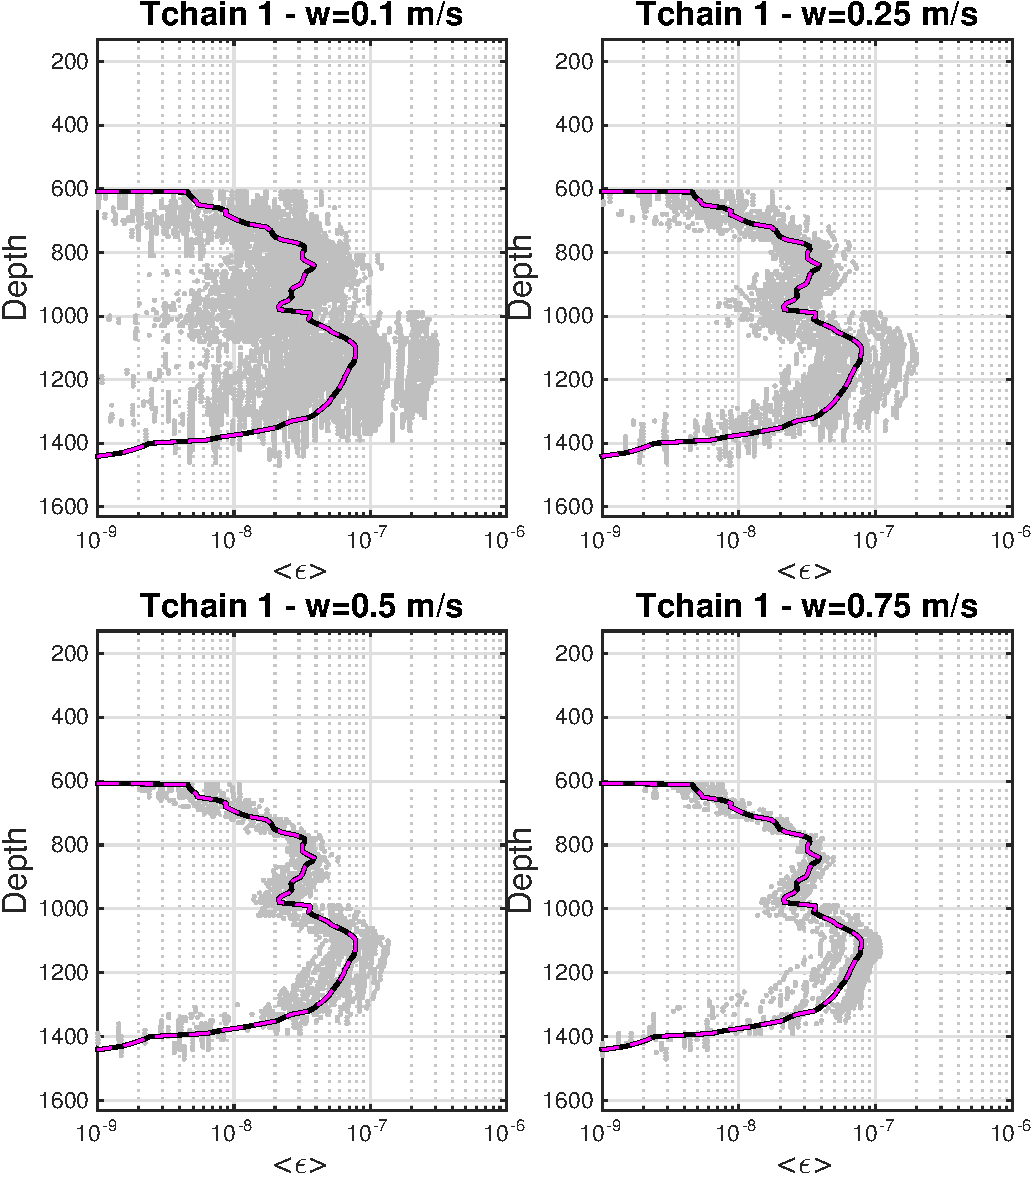
\includegraphics[scale=0.8]{Tchain1_UnderSamp_4speeds.pdf}
%\caption{Time-averaged depth profiles of epsilon for different profiling speeds. Black is the true value using all Tchain data. Gray are mean profiles using only the Tchain profiles at times of resampled profiles (time at center of resampled profile). Each gray line is for profiles shifted slightly in time since phasing of sampling is unknown. Magenta is the mean of all gray lines.}
%\label{}
%\end{figure}
%
%\begin{figure}[htbp]
%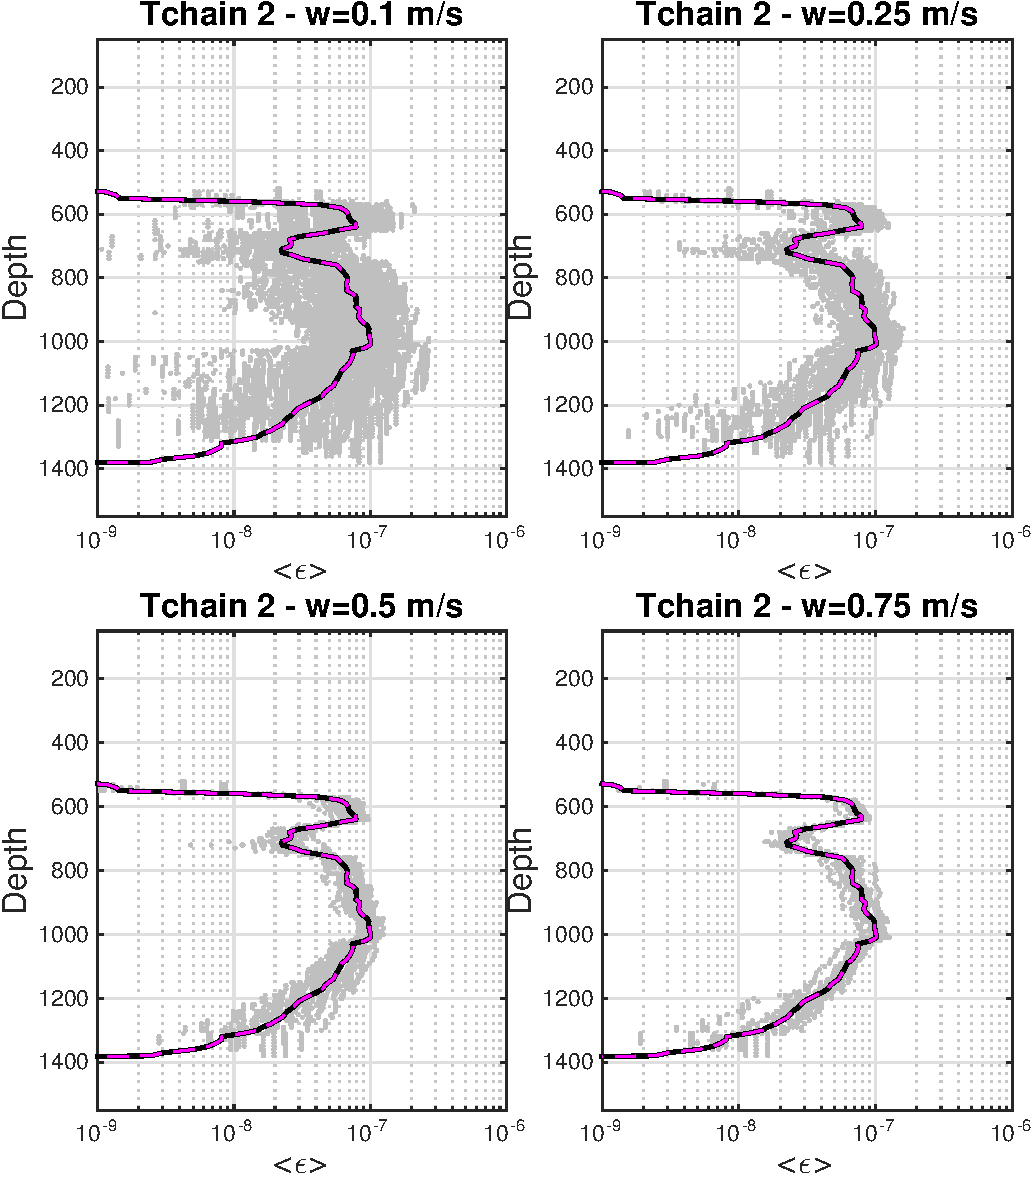
\includegraphics[scale=0.8]{Tchain2_UnderSamp_4speeds.pdf}
%\caption{Time-averaged depth profiles of epsilon for different profiling speeds. Black is the true value using all Tchain data. Gray are mean profiles using only the Tchain profiles at times of resampled profiles (time at center of resampled profile). Each gray line is for profiles shifted slightly in time since phasing of sampling is unknown. Magenta is the mean of all gray lines.}
%\label{}
%\end{figure}

\begin{figure}[htbp]
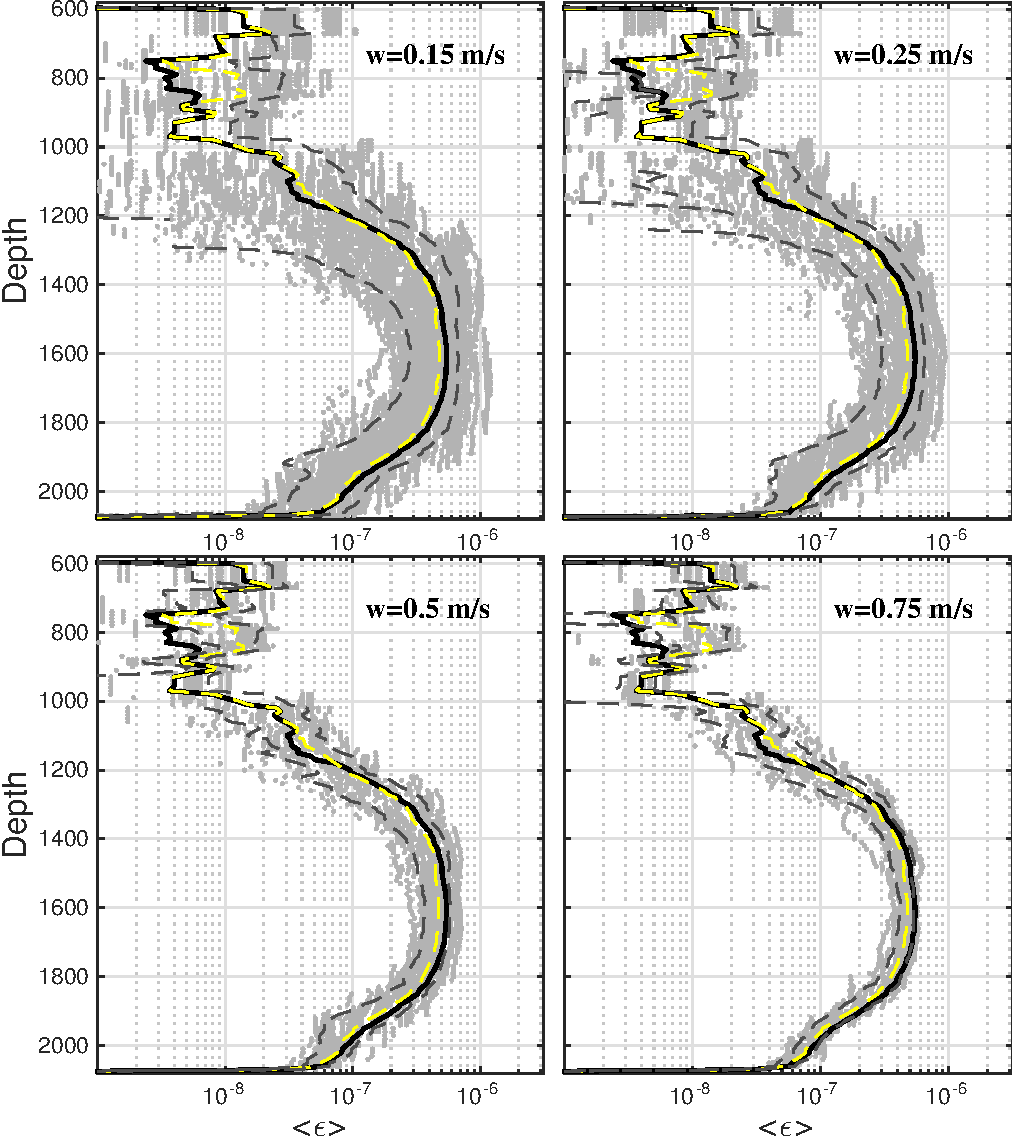
\includegraphics[scale=0.8]{Tchain3_UnderSamp_4speeds.pdf}
\caption{Time-averaged depth profiles of epsilon for different profiling speeds. Black is the true value using all Tchain data. Gray are mean profiles using only the Tchain profiles at times of resampled profiles (time at center of resampled profile). Each gray line is for profiles shifted slightly in time since phasing of sampling is unknown. Magenta is the mean of all gray lines.}
\label{}
\end{figure}

\begin{figure}[htbp]
\includegraphics[scale=0.8]{Tchain4_UnderSamp_4speeds.pdf}
\caption{Time-averaged depth profiles of epsilon for different profiling speeds. Black is the true value using all Tchain data. Gray are mean profiles using only the Tchain profiles at times of resampled profiles (time at center of resampled profile). Each gray line is for profiles shifted slightly in time since phasing of sampling is unknown. Magenta is the mean of all gray lines.}
\label{}
\end{figure}



\newpage
\clearpage
%~~~~~~~~~~~~~~~~~~~~~~~~~~~~~~~~~~~~~~~~~~~~~~~~~~~~~~
\section{Effect of non-instantaneous profiles}
%~~~~~~~~~~~~~~~~~~~~~~~~~~~~~~~~~~~~~~~~~~~~~~~~~~~~~~

%PlotResampResults12Nov.m

\begin{figure}[htbp]
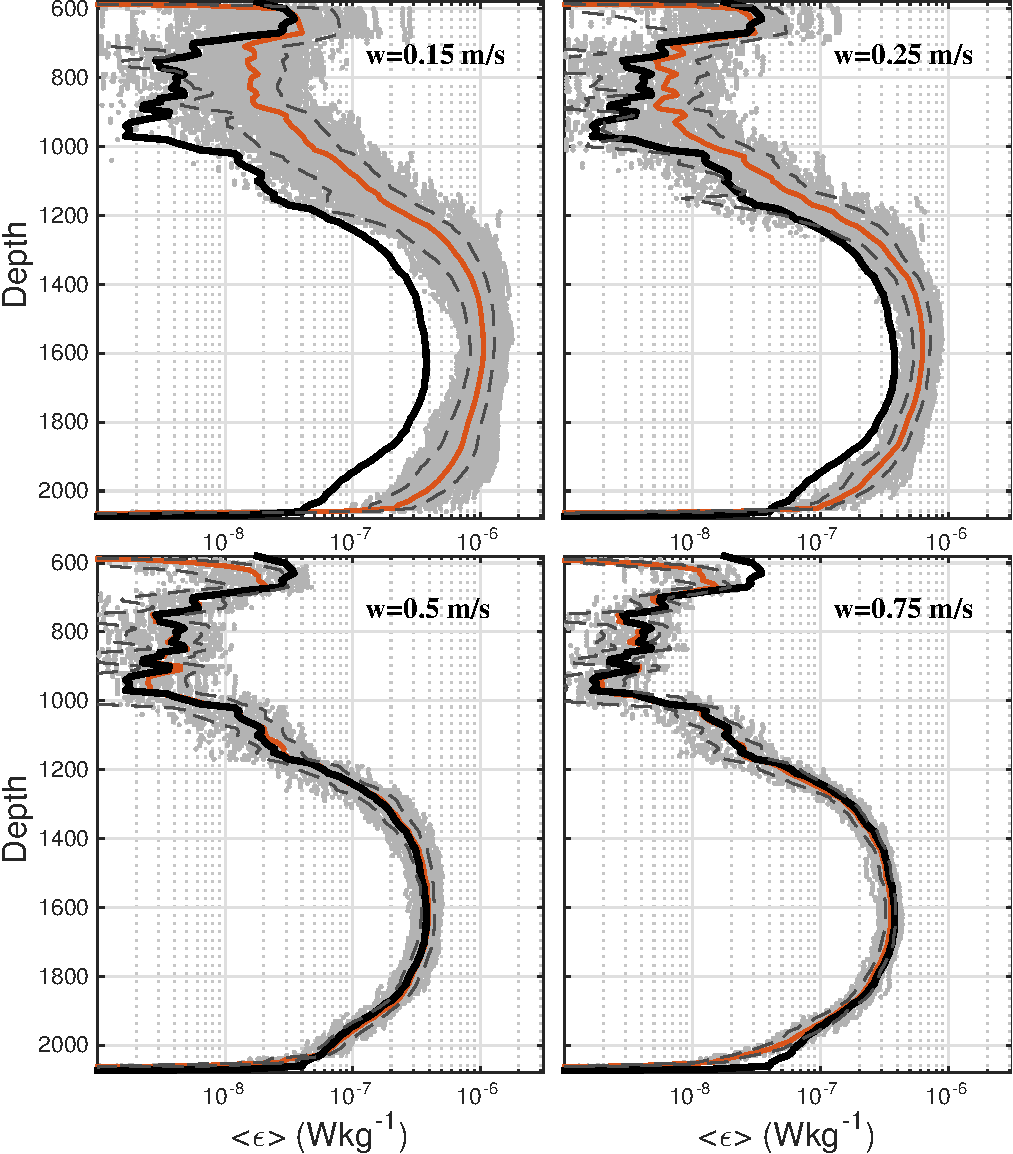
\includegraphics[scale=0.8]{Tchain3_Resamp_EpsvsDepth_DiffSpeeds_2X2.pdf}
\caption{}
\label{}
\end{figure}

\begin{figure}[htbp]
\includegraphics[scale=0.8]{Tchain4_Resamp_EpsvsDepth_DiffSpeeds_2X2.pdf}
\caption{}
\label{}
\end{figure}


\begin{figure}[htbp]
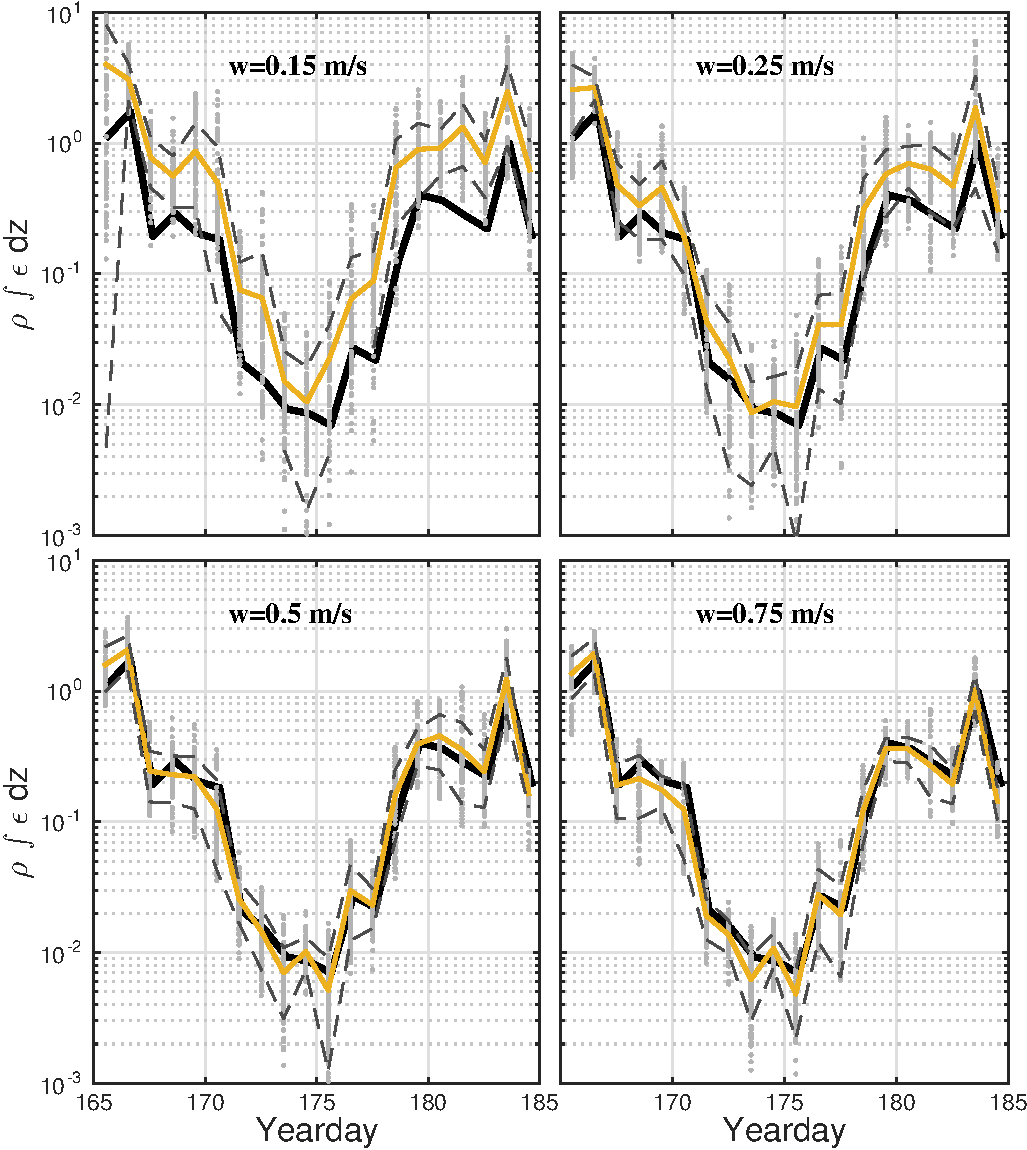
\includegraphics[scale=0.8]{Tchain3_Resamp_IntEpsvsTime_DiffSpeeds_2X2.pdf}
\caption{}
\label{}
\end{figure}

\begin{figure}[htbp]
\includegraphics[scale=0.8]{Tchain4_Resamp_IntEpsvsTime_DiffSpeeds_2X2.pdf}
\caption{}
\label{}
\end{figure}


% PlotResamp_CTDscenario.m
%~~~~~~~~~~~~~~
\subsection{CTD scenario}

\begin{figure}[htbp]
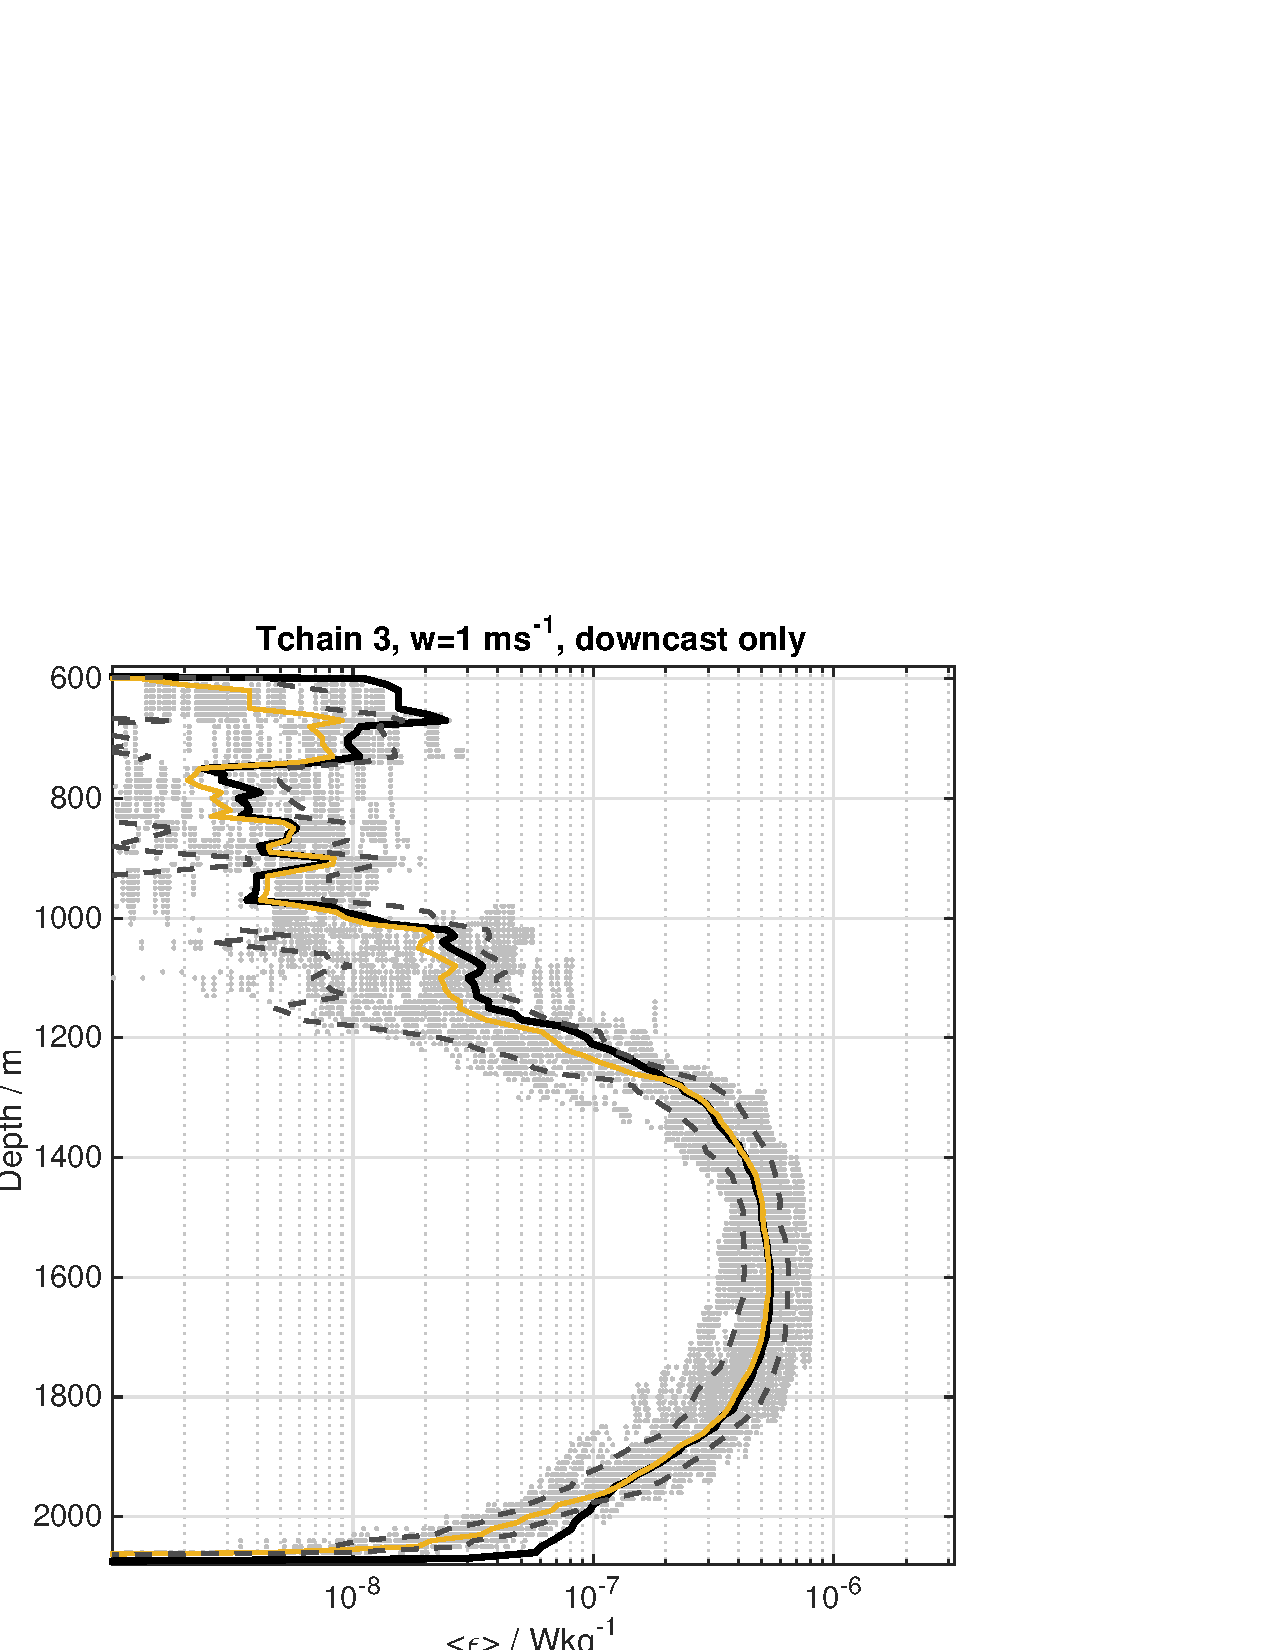
\includegraphics[scale=0.8]{Tchain3_Resamp_EpsvsDepth_CTDscenario.pdf}
\caption{Simulated sampling of T-chain 3 by a CTD package profiling at $1m/s$, using only downcasts. Dashed lines show $\pm$ 1 standard deviation.}
\label{}
\end{figure}

\begin{figure}[htbp]
\includegraphics[scale=0.8]{Tchain4_Resamp_EpsvsDepth_CTDscenario.pdf}
\caption{Simulated sampling of T-chain 4 by a CTD package profiling at $1m/s$, using only downcasts. Dashed lines show $\pm$ 1 standard deviation.}
\label{}
\end{figure}


\newpage
\clearpage
%~~~~~~~~~~~~~~~~~~~~~~~~~~~~~~~~~~~~~~~~~~~~~~~~~~~~~~
\section{Difference between actual and resampled overturn sizes}
%~~~~~~~~~~~~~~~~~~~~~~~~~~~~~~~~~~~~~~~~~~~~~~~~~~~~~~


Histograms of the difference between true and resampled overturn sizes look symmetric. As the profiling speed is increased, the distribution becomes narrower.

See \verb+PlotResampVsTrue_direct.m+.


\begin{figure}[htbp]
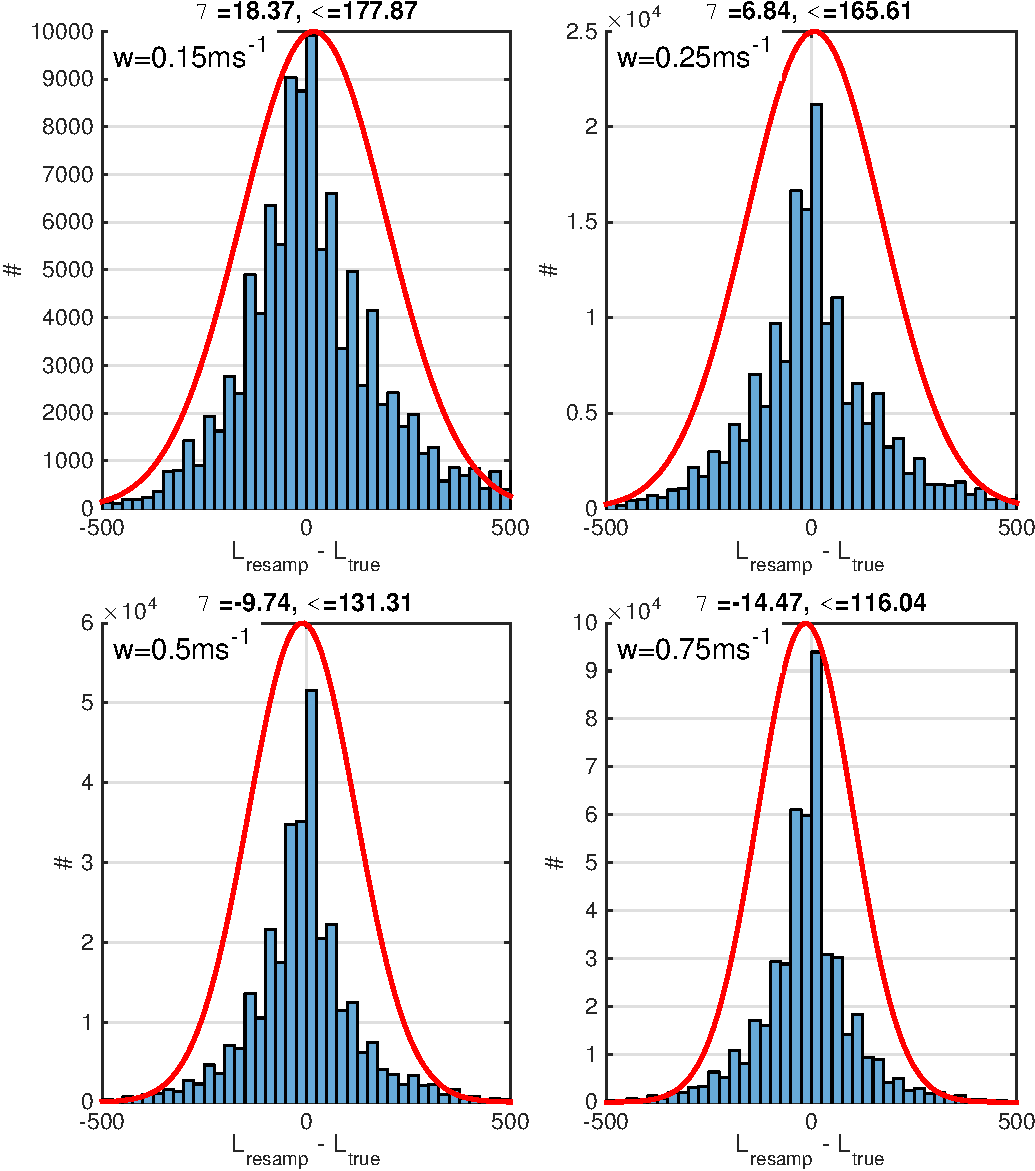
\includegraphics[scale=0.8]{Tchain3_LtDifHist_4Cases.pdf}
\caption{Histograms of the difference between true and resampled overturn sizes at T-chain 3 for 4 different speeds. Red curves are fit to normal distribution (scaled to fit on axes).}
\label{}
\end{figure}

\begin{figure}[htbp]
\includegraphics[scale=0.8]{Tchain4_LtDifHist_4Cases.pdf}
\caption{Histograms of the difference between true and resampled overturn sizes at T-chain 4 for 4 different speeds.Red curves are fit to normal distribution (scaled to fit on axes).}
\label{}
\end{figure}



\newpage
\clearpage
%~~~~~~~~~~~~~~~~~~~~~~~~~~~~~~~~~~~~~~~~~~~~~~~~~~~~~~
\section{Difference in epsilon vs magnitude.}
%~~~~~~~~~~~~~~~~~~~~~~~~~~~~~~~~~~~~~~~~~~~~~~~~~~~~~~

It appears that the error between resampled and true epsilon is proportional to the magnitude of the true epsilon.

\begin{figure}[htbp]
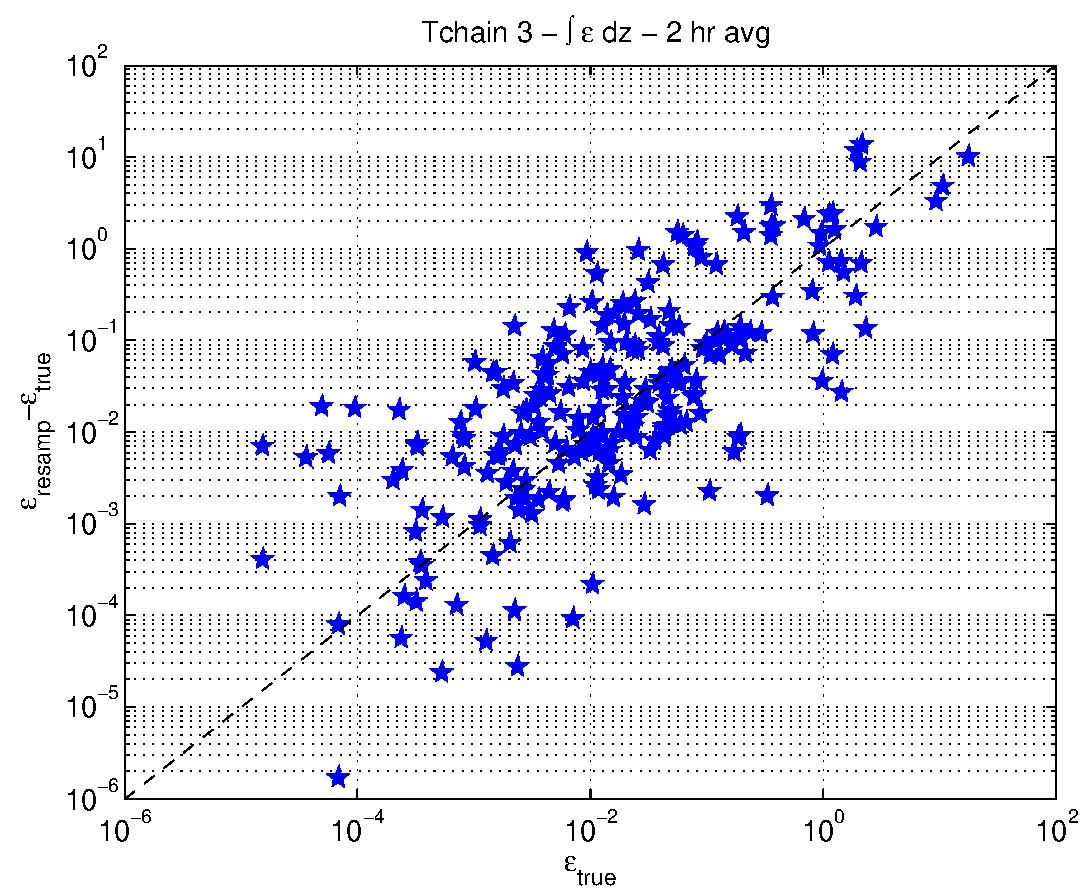
\includegraphics[scale=0.8]{Tchain3_IntEps_ErrorvsTrue.pdf}
\caption{Scatter plot of the difference between resampled and true depth-integrated epsilon versus the true epsilon.}
\label{}
\end{figure}

\begin{figure}[htbp]
\includegraphics[scale=0.8]{Tchain4_IntEps_ErrorvsTrue.pdf}
\caption{Scatter plot of the difference between resampled and true depth-integrated epsilon versus the true epsilon.}
\label{}
\end{figure}



\newpage
\clearpage
%~~~~~~~~~~~~~~~~~~~~~~~~~~~~~~~~~~~~~~~~~~~~~~~~~~~~~~
\section{LES Model at N2}
%~~~~~~~~~~~~~~~~~~~~~~~~~~~~~~~~~~~~~~~~~~~~~~~~~~~~~~

Main directory is \verb+/IWISE/Analysis/S9/Dissipation/OverturnsBiases/LES+. 

Data and m-files:
\begin{itemize}
\item Data (except for dissipation) are in \verb+N2_all.mat+, which is a cell array with one cell for each time.
\item  I combine this data into a depth-time structure in \verb+Make_LES_N2_DepthTime.m+ and save as \verb+N2_depth_time.mat+.
\item  Dissipation (directly computed from velocity shear) data are in \verb+N2turbdiss_ZT.dat+. 
\item I read this into matlab and make into a depth-time structure in \verb+Import_N2_LES_diss.m+.
\item Compute OT for the true LES data in \verb+Compute_OT_LES.m+.	
\item In \verb+CompareLES_N2_OTvsDiss.m+ I compare epsilon from overturns to the direct epsilon computed by Masoud (using shear). 
\item I then resample LES data and compute overturns in \verb+Resample_LES_OT.m+.
\end{itemize}


Summary of LES overturns findings so far (see LES section of notes for details).
\begin{itemize}
\item Epsilon from overturns is about 1 order of magnitude larger than directly computed epsilon. Masoud found something similar also.
\item Masoud assumed Lt equals Lo; should ask him if he compared the two.
\item Resampled overturns don't appear to have much of a bias at any speed. This differs from what I found at the T-chains.
\item N2 is more on top of ridge, maybe it is different at that location?
\item Still want to do comparison at Tchain locations also to see if results are similar.
\end{itemize}

% Make_LES_N2_DepthTime.m
\begin{figure}[htbp]
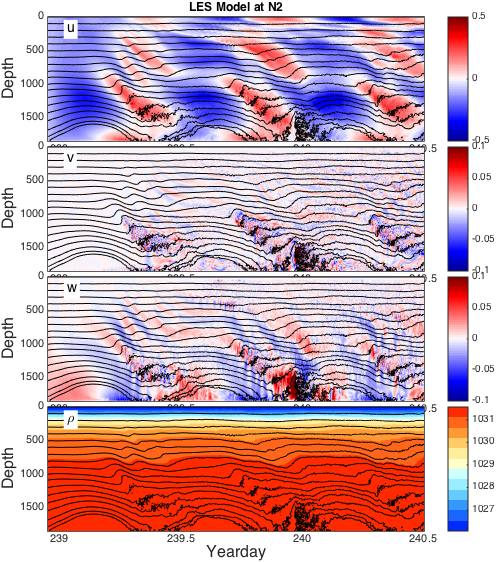
\includegraphics[scale=0.8]{LES_N2_summary.png}
\caption{LES model data at N2 location. Data have been interpolated onto an evenly spaced depth grid (10m).}
\label{}
\end{figure}

% Compute_OT_LES.m
\begin{figure}[htbp]
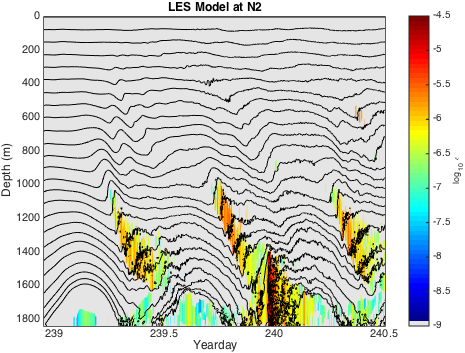
\includegraphics[scale=0.8]{LES_N2_OTeps.png}
\caption{Epsilon computed from overturns in LES model data at N2 location.}
\label{}
\end{figure}

% CompareLES_N2_OTvsDiss.m
\begin{figure}[htbp]
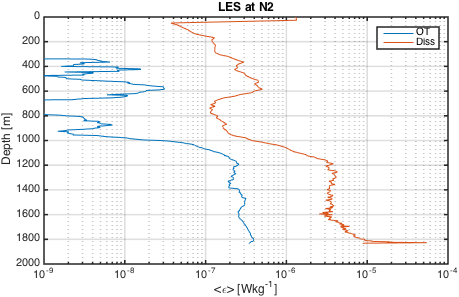
\includegraphics[scale=0.8]{LES_N2_OTvsDirectProfiles.png}
\caption{Time-mean epsilon computed from overturns (OT) and directly from shear (Diss) in LES model data at N2 location.}
\label{}
\end{figure}





\newpage
\clearpage
%~~~~~~~~~~~~~~~~~~~~~~~~~~~~~~~~~~~~~~~~~~~~~~~~~~~~~~
\section{T-tide Moorings}
%~~~~~~~~~~~~~~~~~~~~~~~~~~~~~~~~~~~~~~~~~~~~~~~~~~~~~~

Looking at `T2' mooring from T-tide cruise. Thermistors spaced 10-30m apart measured the bottom 600m.

\subsection{Data and codes}

Main directory is \verb+/IWISE/Analysis/S9/Dissipation/OverturnsBiases/Ttide+. 

\begin{itemize}
\item Original data is in \verb+/Users/Andy/Dropbox/ttide_jn/T2_short_timeseries.mat+. This is a rough processed dataset that JN made for me to do this resampling analysis. Not corrected for mooring knockdown? Absolute depths not correct but probably doesn't matter for this.
\item \verb+ExamineT2.m+ - Quick look at data etc. (see Figure \ref{T2temp}).
\item \verb+Make_T2_grid.m+  - Interpolate T2 to evenly spaced depth and time grid.
\item \verb+ComputeOverturnsT2_gridded.m+ - Compute overturns (all profilies, not resampled).
\item \verb+ComputeOverturnsT2_gridded.m+ - Compute overturns (all profilies, not resampled) using gridded data.
\item \verb+ResampleT2.m - Resampe data to simulate profiling instrument, and comptue overturns for resampled data etc.
\item \verb+CombineResampTestCases_T2.m+ - Combine resampled data into one structure for ensemble.
\item \verb+ PlotResampT2.m+ - Plot results of resampling etc.
\end{itemize}


%~~~~~~~~~~~~~~
\subsection{Data Overview}
 
Figure \ref{T2temp}
 
% PlotSummaryData.m
\begin{figure}[htbp]
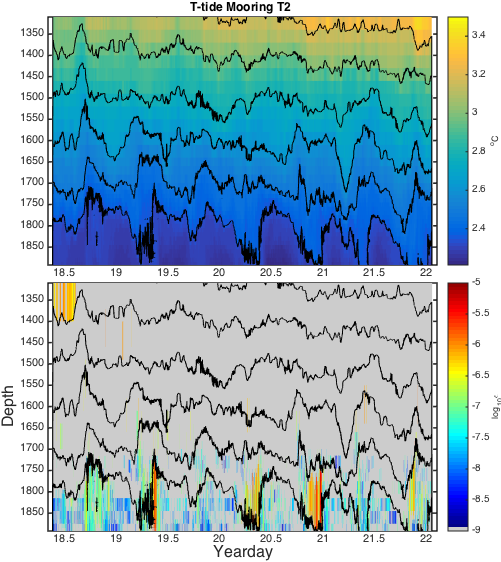
\includegraphics[scale=0.8]{T2_Temp_and_Eps.png}
\caption{Temperature, epsilon from overturns and isotherms at T-tide mooring T2.}
\label{T2temp}
\end{figure}


% PlotSummaryData.m
\begin{figure}[htbp]
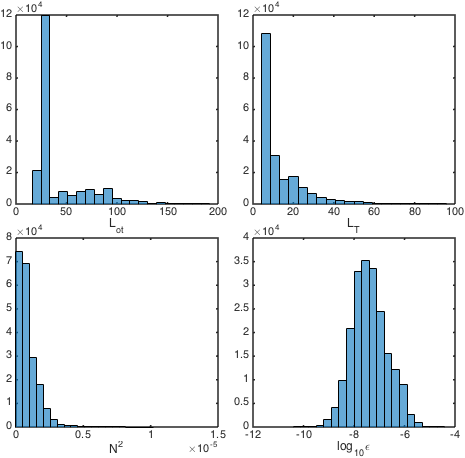
\includegraphics[scale=0.8]{T2_OThist_raw.png}
\caption{Histograms of overturn quanitites at T2 (raw ungridded data).}
\label{}
\end{figure}



\clearpage

%~~~~~~~~~~~~~~
\subsection{Effect of Gridding on Overturns}

I noticed that interpolating the data onto an evenly space depth/time grid affected the mean epsilon profile computed from overturns. So I investigated more to determine how much the effect was and what causes it.

Summary:
\begin{itemize}
\item It is mainly the gridding in depth, gridding in time doesn't have much of an effect. \item Mean gridded profiles of epsilon are all smaller than the raw profile. 
\item They don't go in order of increasing dz.
\end{itemize}


% CompareDiffGridding.m
\begin{figure}[htbp]
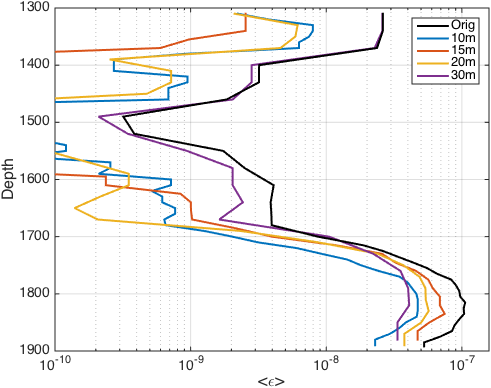
\includegraphics[scale=0.8]{T2_EpsProfile_diffdz.png}
\caption{Time-mean profiles of epsilon for different depth gridding of data. .}
\label{}
\end{figure}



\clearpage

%~~~~~~~~~~~~~~
\subsection{Effect of Resampling on Overturns}



% PlotResampT2.m
\begin{figure}[htbp]
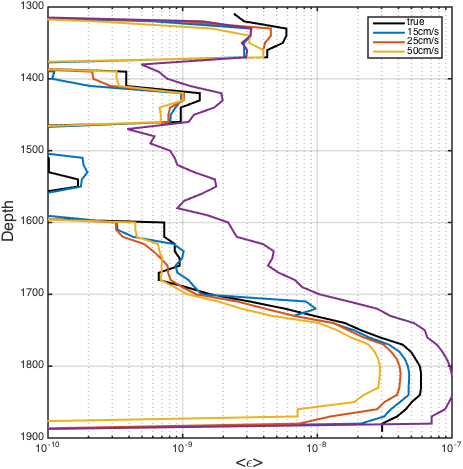
\includegraphics[scale=0.8]{T2_EpsProfResamp.png}
\caption{Time-mean profiles of epsilon for different resampling speeds.}
\label{}
\end{figure}



\newpage
\clearpage
%~~~~~~~~~~~~~~~~~~~~~~~~~~~~~~~~~~~~~~~~~~~~~~~~~~~~~~
\section{Daily Notes}
%~~~~~~~~~~~~~~~~~~~~~~~~~~~~~~~~~~~~~~~~~~~~~~~~~~~~~~



\clearpage
\newpage
%~~~~~~~~~~~~~~~~~
\subsection{23 Nov. 2015}

Again getting back to this... Need to try computing a `turbulent velocity scale' to see if we can identify biased overturns etc...Looks like I started trying this in \verb+Misc16Mar.m+.  Working with new script \verb+Correct_Resampled_Eps.m+. I compute a `turbulenty velocity scale' as $w_t=L_TN$, which follows from

\begin{eqnarray}
\epsilon=L_{T}^{2}N^3 \\
\epsilon \propto U^3/L
\end{eqnarray}
Then I assume where this is greater than the profiler sampling speed (or some fraction of it), values are biased and throw them out.


% CompareDiffGridding.m
\begin{figure}[htbp]
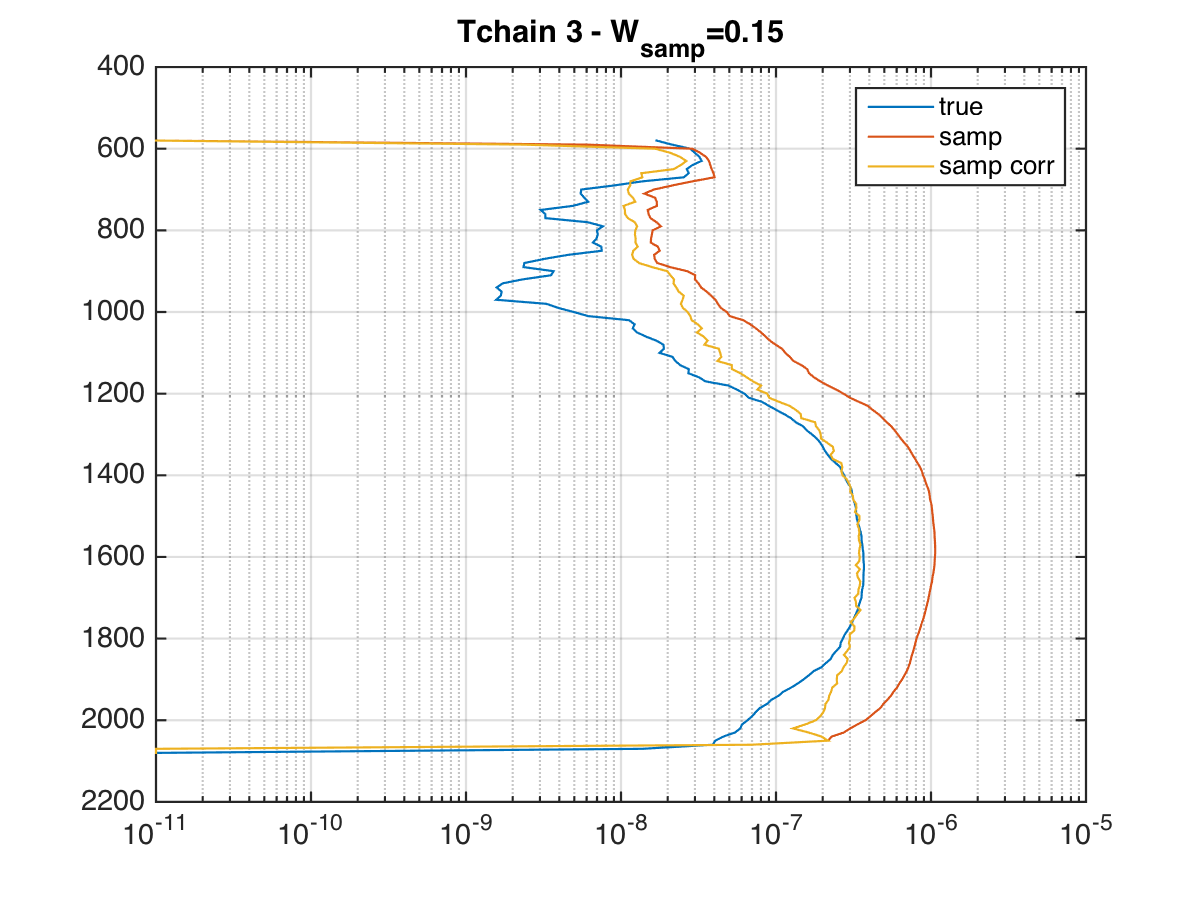
\includegraphics[scale=0.8]{Tchain3_Testnum3_Raw_corr_profiles.png}
\caption{Time-mean profiles of epsilon. For the 'corrected' profile, data where inferred turbulent velocity was greater than 50 percent of the sampling speed were thrown out.}
\label{}
\end{figure}




\clearpage
\newpage
%~~~~~~~~~~~~~~~~~
\subsection{28 May 2015}

Getting back to this after a long break and trying to remember where I left off.  Main script for IWISE Tchain data is: \verb+ResampleProfiler_V2.m+. The core codes to make sample paths and resample are in the folder \verb+/SimProfiler/+




\clearpage
\newpage
%~~~~~~~~~~~~~~~~~
\subsection{23 Mar 2015}


** to do - compare w computed from sampled isotherms to actual w from Tchain data. Try averaging over the period of each profile. Is there any useful correlation?** in Misc16Mar.m

Still trying to think of ways to identify biases in MP data (see 16 mar notes).

Updated list:
\begin{itemize}
\item Find depths of an isopycnal in two consecutive profiles and compute slope (dz/dt). If slope is close to or exceeds the profiling speed, flag as possibly bad. I tried this and unless sampling is fast, this always gives a w that is much smaller than the large values in data.
\item Variation of above: Compute w in a similar way, using profiles before and after each profile. If this w is in same direction as profiler w and exceeds some fraction of the profiler w, flag as possibly bad. Same issues as above, if feature we are trying to capture has timescale shorter than the profiling.
\item Use the actual w measured from the MP. In theory, this works but in practice it is difficult to measure w accurately and would require a significant amount of time working on the code. 
\item Compare consecutive up/down profiles. This effect should be much greater in one, depending on which direction w is in. Problem: the timescale of the overturning patch has to be large enough to be in consecutive profiles. For slower sampling this becomes unlikely.
\item Compare average profiles from up and down casts separately? They should be the same if this effect isn't present. Didn't see any consistent patterns in Tchain 3.
\item Look at shapes of overturns? Is there something consistenly different between real and sampled overturns?
\end{itemize}


\clearpage
\newpage
%~~~~~~~~~~~~~~~~~
\subsection{17 Mar 2015}

Working on new function \verb+ResampleFieldGeneral.m+ to generalize the resampling done in \verb+ResampleProfiler.m+ and make it easy to apply to any dataset. This way I can also modify the code and not have to replicate those modifications in every separate script for each dataset.

Overturns can be added to this REsamp structure with \verb+AddOverturnsToREsamp.m	+


\clearpage
\newpage
%~~~~~~~~~~~~~~~~~
\subsection{16 Mar 2015}

Trying to come with ways to test whether sampling/overturns are biased from proifler data only (ie real life).
\begin{itemize}
\item Find depths of an isopycnal in two consecutive profiles and compute slope (dz/dt). If slope is close to or exceeds the profiling speed, flag as possibly bad. I tried this and unless sampling is fast, this always gives a w that is much smaller than the large values in data.
\item Variation of above: Compute w in a similar way, using profiles before and after each profile. If this w is in same direction as profiler w and exceeds some fraction of the profiler w, flag as possibly bad.
\item Use the actual w measured from the MP. In theory, this works but in practice it is difficult to measure w accurately.
\end{itemize}


* Idea: try taking a woa profile and mode-1 IT w , making synthetic field, sampling to see if we get any false overturns.



\clearpage
\newpage
%~~~~~~~~~~~~~~~~~
\subsection{10 Mar 2015}

Found bug in my resampling code. Was interpolating to the same depth vector for each profile, instead of using alternating up/down (so I think basically using just down profiles). Fixed this in \verb+ResampleProfiler.m+. Doesn't seem to have much effect on the mean profiles or the along-path plots though..

WAIT now there is a bias at Tchain2? Check Tchain1, Ttide mooring also




\clearpage
\newpage
%~~~~~~~~~~~~~~~~~
\subsection{9 Mar 2015}


I made a bunch of plots of epsilon along the actual sampling paths, following JN's suggestion. In a lot of them, at slow sampling speeds there are a few `stripes' of much larger epsilon that I think are largely responsible for the larger mean profiles (ex. Figure \ref{9Mar_1}). It appears that they might at places where the profiler is traveling in the same direction as large isopycnal displacements. Basically it happens in places on depth-time maps where the slope of the sampling path is the same as the slope of the isopycnals... I'm wondering if the bias doesn't show up in other data because the vertical velocities are smaller (so if I sampled even slower, I might see something similar). 


% PlotResampT2.m
\begin{figure}[htbp]
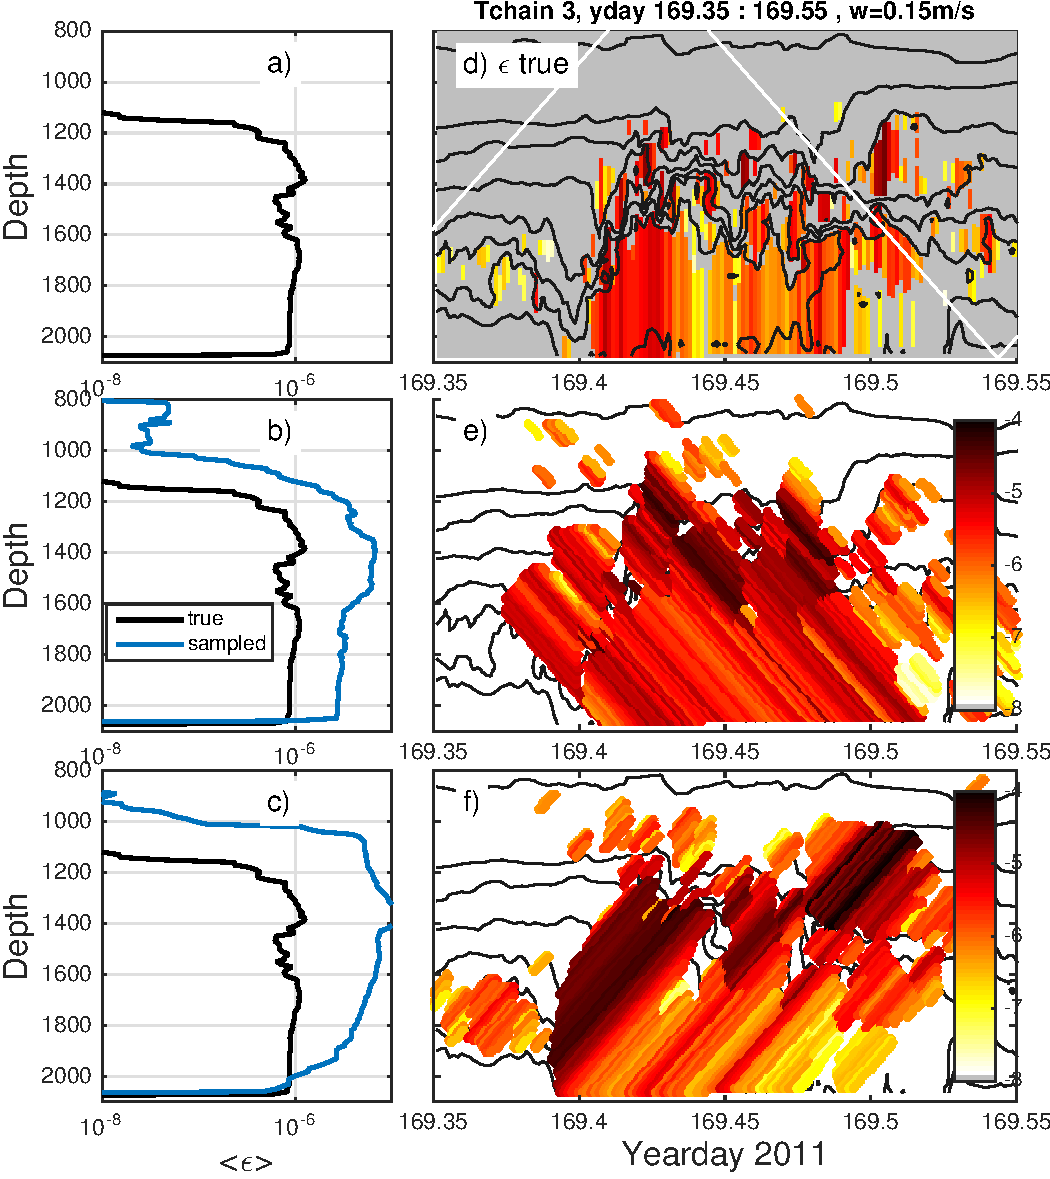
\includegraphics[scale=0.8]{Tchain3_AlongPath_NearDay169_Test_3.pdf}
\caption{(top) True Tchain data. (middle) Epsilon along downward sampling paths. (bottom) Epsilon along upward sampling paths.}
\label{9Mar_1}
\end{figure}


* make same figures for other Tchains.
* if slopes not equal at other tchains, try slower sampling.

What is different about Tchain 3 and 4? Overturns are larger. Overturns last longer and have larger vertical extent. Vertical velocites are larger.


\clearpage
\newpage
%~~~~~~~~~~~~~~~~~
\subsection{4 Mar 2015}


I still don't have a good sense of what specifically causes the bias in epsilon at Tchains 3 and 4. I know that if I remove the `false' overturns (where there wasn't an overturn in true profile but is in real), the bias mostly disappears. I will try looking at this for shorter sections to see why this results in the bias.


\vspace{1cm}

Continuing from yesterday. Figured out bootstrapping with \verb+boot_v5.m+ in mixingsoftware. Wrote \verb+bootstrap_profile.m+ to do this for each depth. Did bootstrapping for mean epsilon profile at Tchain3, the resampled mean profile is well outside the 95\% limits for the true data.


At Ttide T2, where the timeseries is only a few days, the separation between the resampled mean and the true confidence limits is smaller. When I do bootstrap conf lims for true and resampled, they overlap for most of the cases. So I don't think I can really say whether there is a bias here. A longer timeseries would help. 


\clearpage
\newpage
%~~~~~~~~~~~~~~~~~
\subsection{3 Mar 2015}

Need to compute bootstrap confidence limits for mean dissipation profiles (true). Are the resampled profiles in or outside these limits? If timeseries is short (T2?), conf. limits might be too big to say if there is a bias or not...




\clearpage
\newpage
%~~~~~~~~~~~~~~~~~
\subsection{2 Mar 2015}

Doing analysis for JN's Ttide mooring `T2'. See details in section above. Noticing that gridding the data makes a sizable difference in mean epsilon profiles. Seems to be mostly the depth gridding. Another complication...





\clearpage
\newpage
%~~~~~~~~~~~~~~~~~
\subsection{27 Feb 2015}


* shortsectionsresamp... plot timeseries

Decdied to look at Tchains 1 and 2 again. I had assumed they didn't capture dissipation well becuase overturns were smaller there. But maybe the same bias just doesn't happen there? There doesn't seem to be any bias at Tchain1, but its possible that overturns there are smaller and not well resolved to begin with...




\clearpage
\newpage
%~~~~~~~~~~~~~~~~~
\subsection{25 Feb 2015}

I did resampling for the complete timeseries (two more spring tides), results and biases seem to hold. If anything, bias during 3rd spring might be larger.

\vspace{1cm}

I extended the resampling at Tchains 3 and 4 to cover two more spring tides. Results are similar.

\vspace{1cm}

I think I really need to do the analysis at some other locations. Might be dependent on the location and turbulence regime etc..

\clearpage
\newpage
%~~~~~~~~~~~~~~~~~
\subsection{24 Feb 2015}

Summary of LES overturns findings so far (see LES section of notes for details).
\begin{itemize}
\item Epsilon from overturns is about xx times larger? than directly computed epsilon. Masoud found something similar also.
\item Masoud assumed Lt equals Lo; should ask him if he compared the two.
\item Resampled overturns don't appear to have much of a bias at any speed. This differs from what I found at the T-chains.
\item N2 is more on top of ridge, maybe it is different at that location?
\item Still want to do comparison at Tchain locations also to see if results are similar.
\end{itemize}


\clearpage
\newpage
%~~~~~~~~~~~~~~~~~
\subsection{19 Feb 2015}

Started looking at the LES data at N2 from Sutanu and Masoud. Think i've figured out the scaling etc. and did a first pass at computing overturns. The model data is potential density (not temp and salinity) so I made a modified overturns code to use that as input. I also needed to make a modified function (from \verb+sw_bfrq.m+) to calculate buoyancy frequency from potential density instead of t and s (\verb+Nsq_pden.m+). Nsq computed via the two differes a little bit, I think because of the way the averaging is done. But for my purposes here it shouldn't matter as long as I use the same method.

* working on \verb+Resample_LES_OT.m+

\clearpage
\newpage
%~~~~~~~~~~~~~~~~~
\subsection{18 Feb 2015}

It seems like if I look at histograms of all epsilon, true and sampled aren't very different. But the profiles of average or integrated epsilon differ? Try looking at one depth?


What happens to averages if I replace 1e-11 with zeros? is it senstive to choice of this value?


\clearpage
\newpage
%~~~~~~~~~~~~~~~~~
\subsection{16 Feb 2015}

Need to be careful about looking at histograms/scatter plots of thorpe scales and overturn sizes etc.. Each depth value in an overturn is given the same value, so larger overturns might be weighted more than smaller ones. 

\vspace{1cm}


Got some LES model data from Masoud/Sutanu at N2 location and started looking at it:
\verb+PlotLES_N2.m+. Need to figure out how to scale potential density. Also will need to adapt overturns code to input potential density instead of t and s.


\vspace{1cm}

I have modified overturns code to return displacements, N2, etc. so I can do more diagnostics. Plan to compare d, N2, dT/dz etc. to try to learn more about what is causing bias in epsilon between true and resampled.


\vspace{1cm}

Modified the resampling a bit to use the exact number of shifts to cover 1 profiling period isntead of using 100 for each. This number is less than 100 for all speeds except $0.15$m/s, for which it is 166 so might have been undersampled. I compared mean profiles with the different numbers and the differences are small (much less than the bias compared to true).


\clearpage
\newpage
%~~~~~~~~~~~~~~~~~
\subsection{13 Feb 2015}

We know that the resampled epsilon (averaged) is biased high, but why? Compare true and resampled temp, N2, dTdz etc. to see if we can see what is the dominant cause.

\vspace{1cm}

I had thought that $L_{ot}$ in the overturns code was the thorpe displacements, but it is actually the patch size (the vertical size of each overturning region). Because this value is assigned to each point within each region, it might be misleading to look at statistics of it, since larger regions will be weighted more heavily?

\vspace{1cm}

I think I need to spend a little time working on the overturns code today to (1) make sure I completely understand what is doing (2) make it more transparent and well-documented (3) return additional variables and make summary plots, and be able to vary parameters more easily.

\vspace{1cm}

I want code to:

\begin{itemize}
\item Return re-ordering displacements
\item have a parameters structure
\item Generic plotting routines for profiles and individual overturns
\item return sorted profiles and N (needed for plotting above..)
\item Be readable and understandable by new users
\item Return list of patch sizes and Thorpe scales (one for each overturning region, not one for each point) for statistics.
\end{itemize}



\clearpage
\newpage
%~~~~~~~~~~~~~~~~~
\subsection{11 Feb 2015}

I decided I need to go through the overturns code to clean it up and better understand everything it is doing. I think that Lot is actually the patch size, not the individual displacements as I was thinking... Check with JN if the code I have is the best place to start.

\vspace{1cm}

Think I need to summarize what i've found so far and figure out the big picture etc.. 

\vspace{1cm}

\textbf{Big Picture}:

\begin{itemize}
\item Many Thorpe scale estimates of epsilon from moored profilers and CTD profiles.
\item All implicitly make assumption of instantaneous vertical profiles, when really they take some finite time.
\item What is the effect of this assumption on the estimated Thorpe scales and dissipation?
\item Can we diagnose what causes these effects and provide a useful way to apply the results to other locations, in order to quantify the uncertainty in Thorpe scale estimates from profiling instruments?
\end{itemize}


\textbf{Results}:
\begin{itemize}
\item Epsilon (average profiles and depth-integrated time series) computed from resampled Thorpe scales shows a positive bias (averaged over different phases) compared to the true data.
\item The bias is inversely proportional to the sampling speed.
\item For data points where there is an overturn in both the real and sampled data, the distribution of the difference in L looks nearly symmetric (i.e. we are not just always measuring bigger overturns). 
\item There are many `false' overturns, where there was not an overturn in the true profile but there is in the resampled profile. There about half as many cases of the opposite, where there is an overturn in the true profile but not in the resampled profile. 
\item The bias mostly goes away if I remove these `false overturns', suggesting they are the main cause of the bias.
\end{itemize}

\textbf{Remaining Questions and Analysis}
\begin{itemize}
\item I still don't completely understand what exactly is causing the bias. It seems to be largely due to the `false' or mis-assigned overturns. 
\item Can the errors be related to some measure of the background flow (i.e. vertical or horizontal velocity)? 
\item Is vertical or horizontal advection important? (this would depend on the specific flow at the mooring site, and the horizontal gradients).
\item Can the results here be generalized to other locations with different forcing?
\end{itemize}




\clearpage
\newpage
%~~~~~~~~~~~~~~~~~
\subsection{10 Feb 2015}

Trying to plot the contribution to the mean epsilon as a function of the overturn size, to see if the mean epsilon is dominated by a few large overturns etc.. What I did is sort overturns in increasing order, then plot the cumulative sum of epsilon using those indices (T3 in Figure \ref{LepsCont}). In the true data, the contribution from overturns up to about 500m looks pretty linear and accounts for about 65\% of the total. Above that, it increases more sharply as bigger overturns contribute more. The resampled (25cm/s) looks similar up to about 500m, but then is shifter to larger overturns above that. At higher sampling speed, the line approaches the true value. Note however the results at Tchain 4 look different (Fig \ref{LepsContT4}).See \verb+PlotEpsContribVsL.m+


\begin{figure}[htbp]
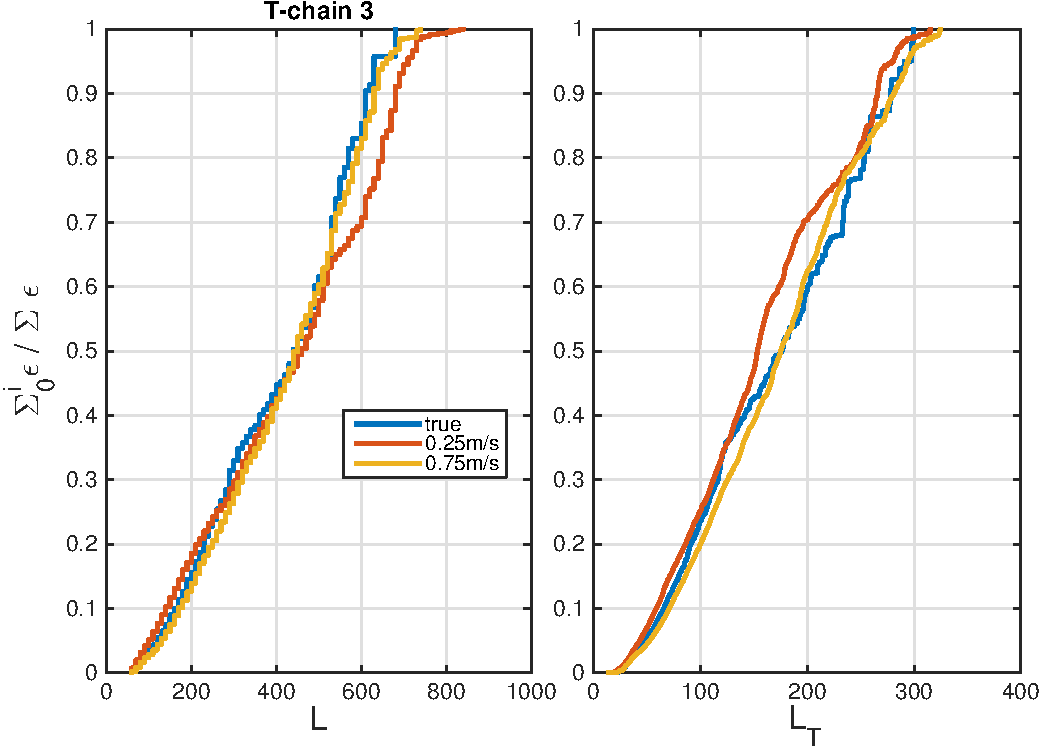
\includegraphics[scale=0.8]{Tchain3_EpsContribVsLot.pdf}
\caption{Cumulative sum of epsilon, sorted by increasing overturn size, versus the overturn size.}
\label{LepsCont}
\end{figure}



\begin{figure}[htbp]
\includegraphics[scale=0.8]{Tchain4_EpsContribVsLot.pdf}
\caption{Cumulative sum of epsilon, sorted by increasing overturn size, versus the overturn size.}
\label{LepsContT4}
\end{figure}



\clearpage
\newpage
%~~~~~~~~~~~~~~~~~
\subsection{5 Feb 2015}

Today I want to examine the relationship between the error or bias and the magnitude of the true dissipation etc.. Is there a linear, consistent relationship? If so, do we understand why? Do we expect it to hold for other locations (if so, could use it to estimate biases). Note that if the error is (linearly) proportional to the true value, this implies that the percent error is constant.

\vspace{1cm}

So why is the scaling different for positive and negative biases? Just because the negative bias can't be more than 100 percent?

\vspace{1cm}

Working in \verb+PlotErrorVsTrueEps.m+ again. If I fit a straight line to the log-log data (abs of all data), I get that the error is proportional to $\epsilon_{o}^{0.6-0.7}$. At slower speeds there seem to be more positive biases than negative, and at higher speeds there are about equal numbers of positive and negative biases. When I do the fit separately for positive and negative biases, I get different exponents. The exponent for the negative biases are close to 1.

\begin{figure}[htbp]
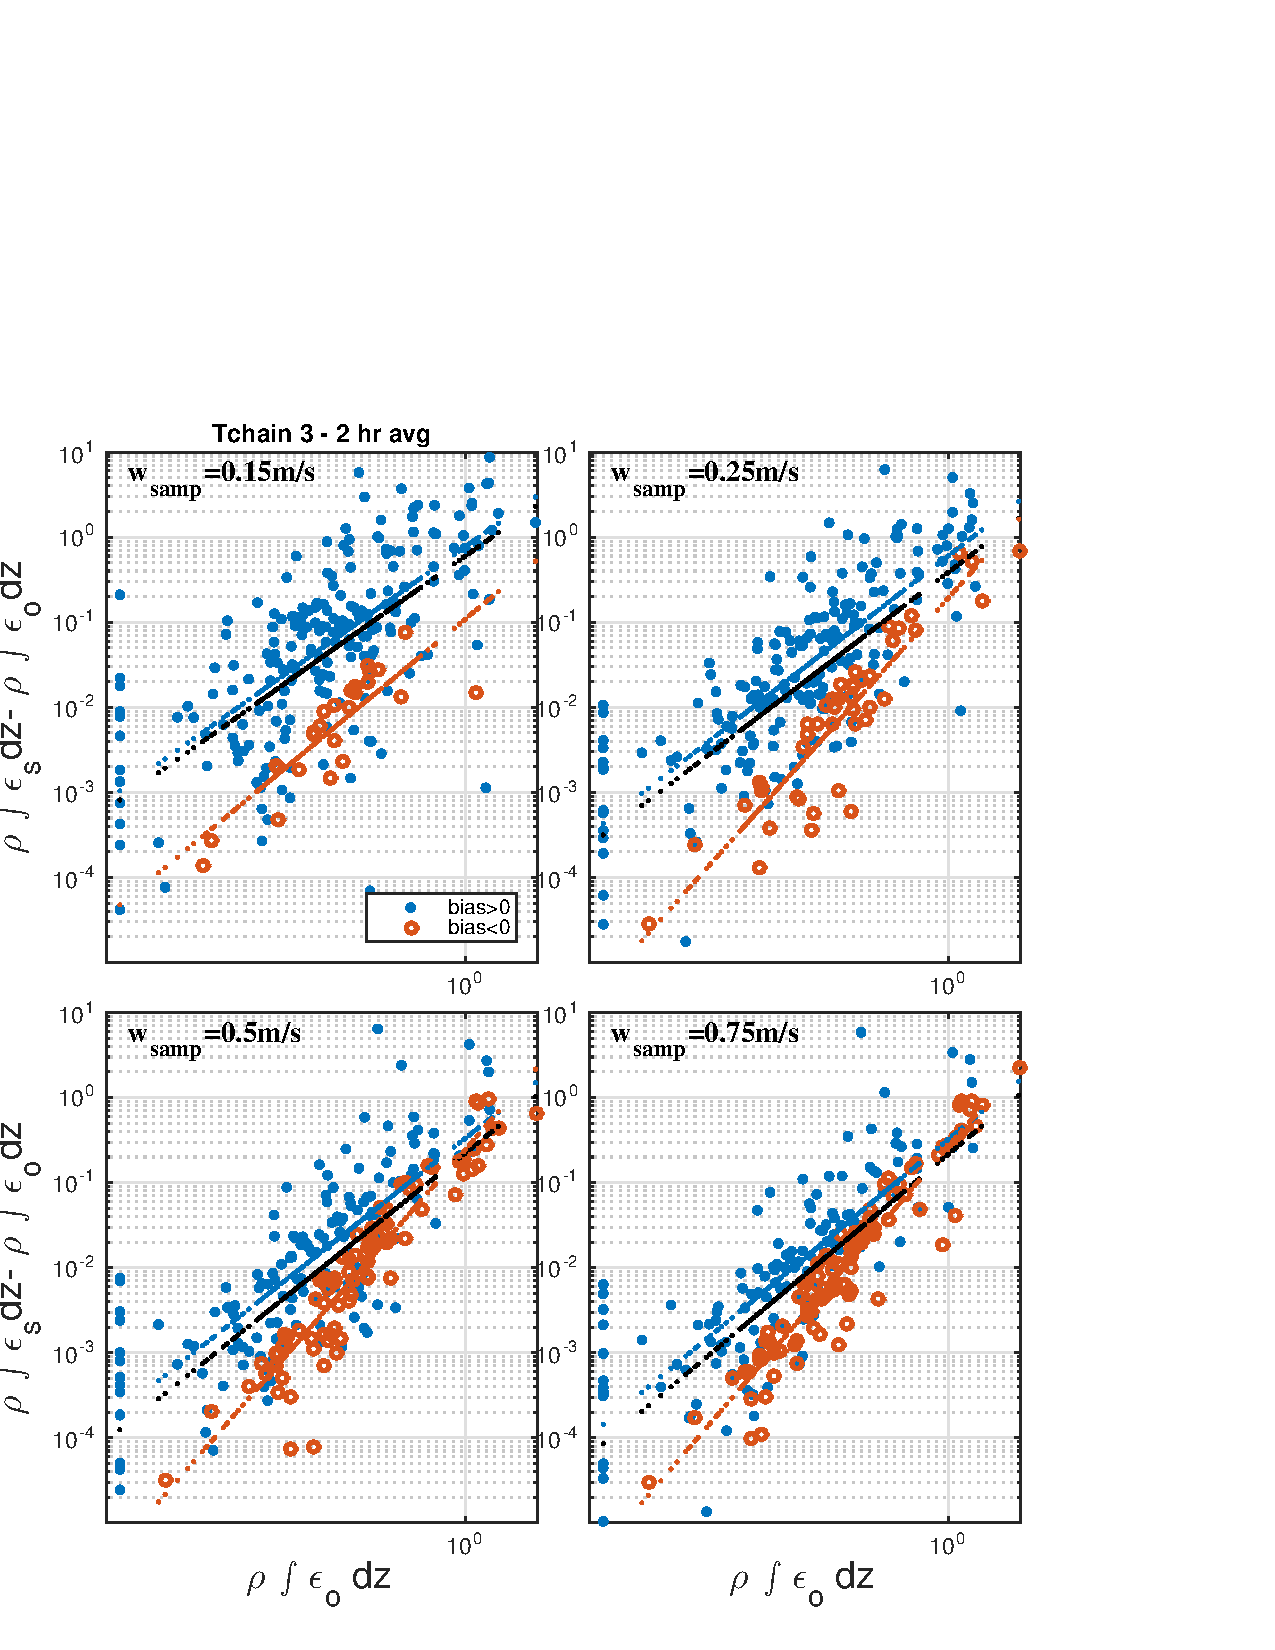
\includegraphics[scale=0.8]{Tchain3_4Speeds_IntEps_ErrorvsTrue.pdf}
\caption{Plots of the error in depth-integrated epsilon (averaged over 2 hours) versus the magnitude of the true epsilon for resampling at 4 different speeds at Tchain3. Positive and negative errors are shown in different colors. Lines show best-fit line for each.}
\label{}
\end{figure}

\vspace{1cm}

I always get mixed up and forget how to plot a straight-line fit to a log-log plot, so i'm writing it here. I use polyfit to fit a straight line to the log of both quantities.
\begin{eqnarray}
\log(Y)=m\log(X) +b\\
10^{\log(Y)}=10^{[m\log(X) +b]}\\
Y=10^{m\log(X)} 10^b\\
Y=10^{\log(X^m)} 10^b\\
Y=X^m 10^b\\
\end{eqnarray}


\clearpage
\newpage
%~~~~~~~~~~~~~~~~~
\subsection{2 Feb 2015}

I'm working in \verb+EvalFalseOverturns.m+ some more, doing the same analysis for depth-integrated epsilon instead of average profiles. The results are essentially the same. 

\vspace{1cm}

I was wondering if somehow my epsilon averages were being screwed up by NaNs where there were no overturns (i.e. having a nan instead of a zero would change the average). There are Nans in L, but any NaNs in epsilon are given a value of 1e-11 so I don't think this is an issue.

\vspace{1cm}

So why are there more false positive overturns than false negative? If it is just that the MP samples turbulence at a different time, it seems like it would be equally likely to sample no turbulence where there actually is...

Are there just more points with overturns than without, so more possibilities for false positives? In the true data, the number of stable points (no overturns) is much larger than the number of points with overturns. About 93 percent of points have no overturns. So there are many more stable points that could become unstable during sampling, than unstable points that could become unstable.

If this is right, however, it means that we probably can't correct the sampled data after the fact since we have no way of knowing which overturns are false?... Maybe looking at persistence (in time) on successive profiles might help? 


\clearpage
\newpage
%~~~~~~~~~~~~~~~~~
\subsection{30 Jan 2015}

Are there more false overturns than false non-overturns (an overturn in the real profile becomes stable in the resampled profile)? I would expect false non-overturns to reduce epsilon, but this doesn't happen so there must be more false overturns? There seem to be about twice as many false overturns as false non-overturns.

\vspace{1cm}

Plot bias vs epsilon magnitude for different speeds on same plot. \verb+PlotErrorVsTrueEps.m+.

\begin{figure}[htbp]
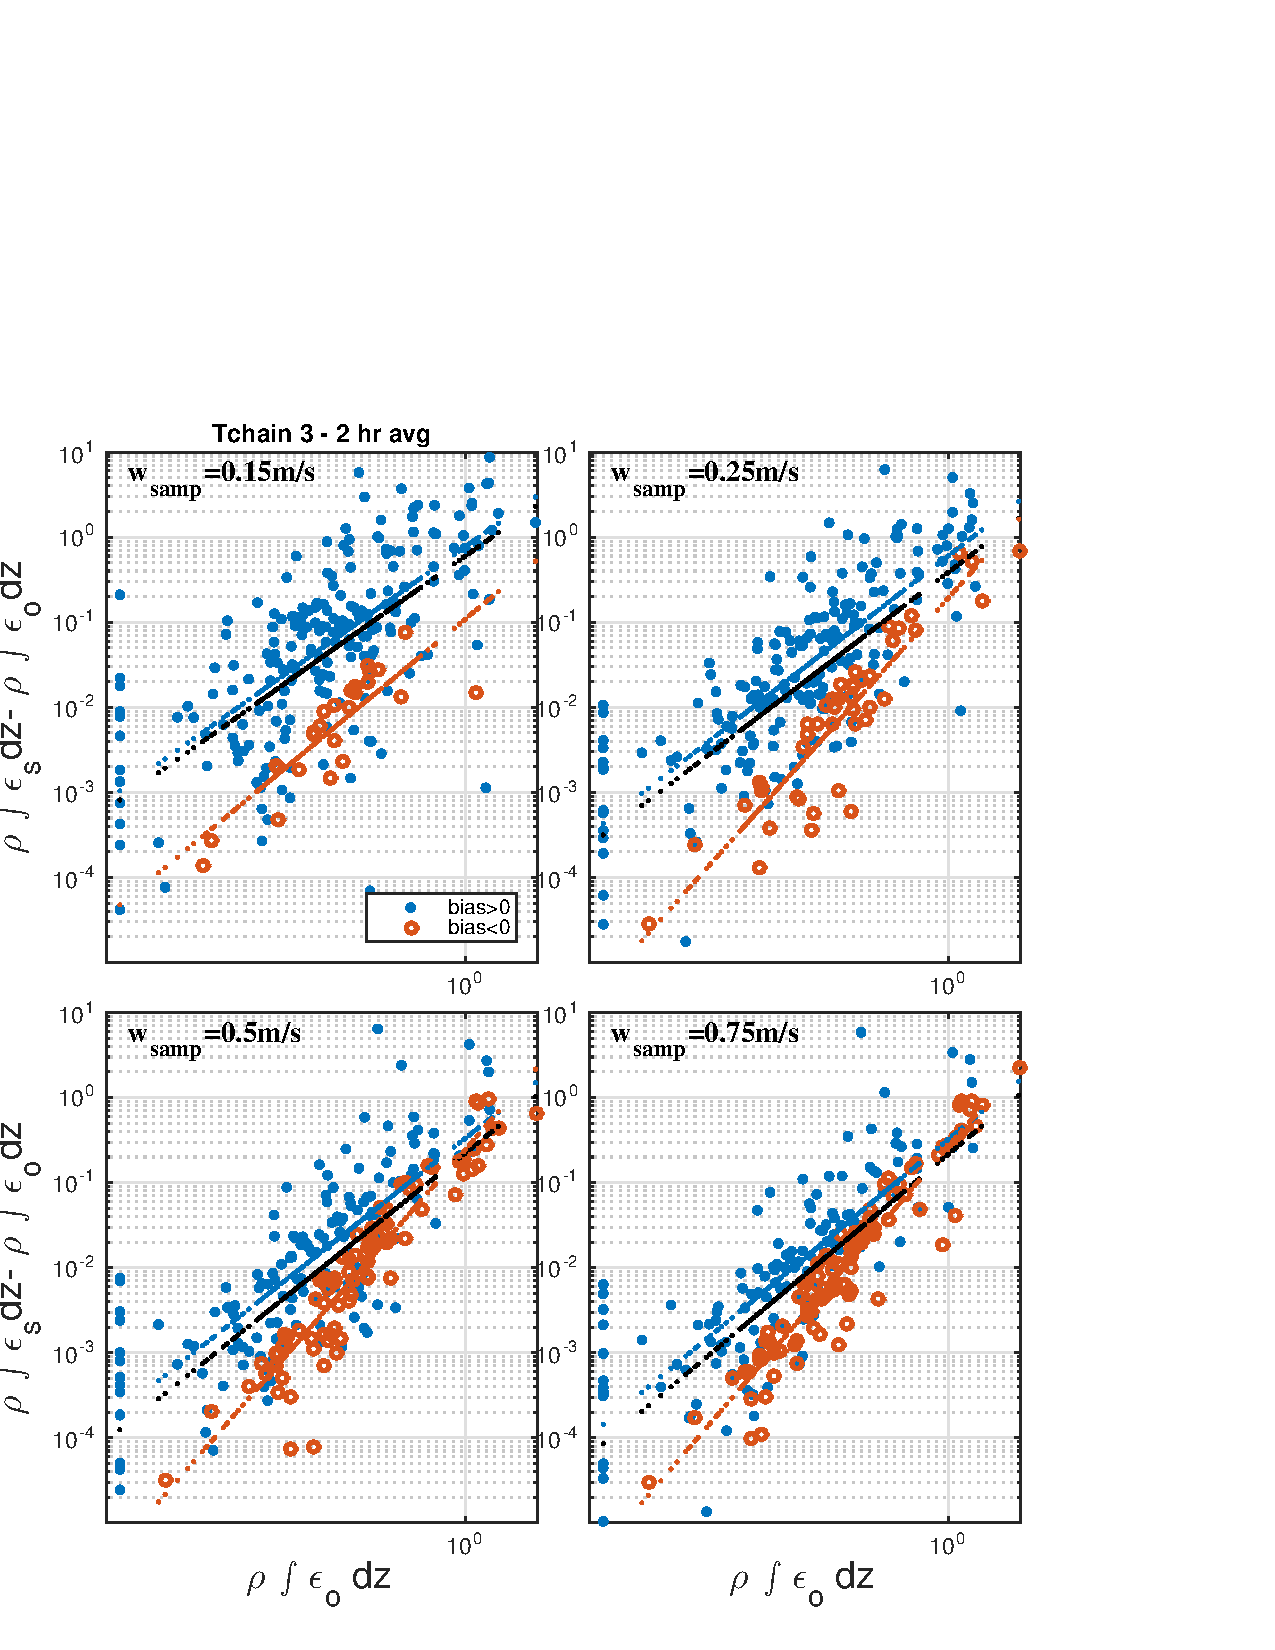
\includegraphics[scale=0.8]{Tchain3_4Speeds_IntEps_ErrorvsTrue.pdf}
\caption{Plots of the error in depth-integrated epsilon (averaged over 2 hours) versus the magnitude of the true epsilon for resampling at 4 different speeds at Tchain3. Positive and negative errors are shown in different colors. Dashed line is slope 1. }
\label{}
\end{figure}

\begin{figure}[htbp]
\includegraphics[scale=0.8]{Tchain4_4Speeds_IntEps_ErrorvsTrue.pdf}
\caption{Plots of the error in depth-integrated epsilon (averaged over 2 hours) versus the magnitude of the true epsilon for resampling at 4 different speeds at Tchain4. Positive and negative errors are shown in different colors. Dashed line is slope 1. }
\label{}
\end{figure}


\vspace{1cm}

Why would the error or bias scale with the true magnitude? Partly because epsilon goes as the square of L? In terms of false overturns, time periods where epsilon is larger are mote turbulent, and profiler is more likely to sample overturns during part of the profile?

\vspace{1cm}

Still don't understand why difference in L vs Ltrue has a negative trend (\verb+ScatterErrorsVsTrue.m+).. 



\newpage
%~~~~~~~~~~~~~~~~~
\subsection{29 Jan 2015}

I want to see how much of an effect false overturns (overturns in the resampled data where there were none in the true profiles) have on the mean profiles of epsilon etc..How many false overturns are there (what percent of total number of points)? How big are they (do they have the same distribution?)? I wrote a new section of code in \verb+EvalFalseOverturns.m+ to examine these questions for the entire ensemble of phases.

\begin{itemize}
\item There are many instances of false overturns (overturns in resampled profiles where there were none in true profiles).
\item The distribution of overturn sizes for false positives looks similar to the total distribution (Figure \ref{T3_FalsePosHist}).
\item Figure \ref{T3_FalsePosProf} shows time-mean profiles (entire ensemble) of epsilon at Tchain 3 for the real, resampled, and resampled w/o false overturns data. This shows that a lot of the increased epsilon in the resampled data is due to false overturns introduced. 
\item Figure \ref{exampleFalsePos} shows an example of how false overturns might be introduced. The true profile (dashed line) is mostly stable, but the resampling samples a period of turbulence that occurs at a later time (but is assigned to the time at the midpoint of the profile). 
\end{itemize}


\begin{figure}[htbp]
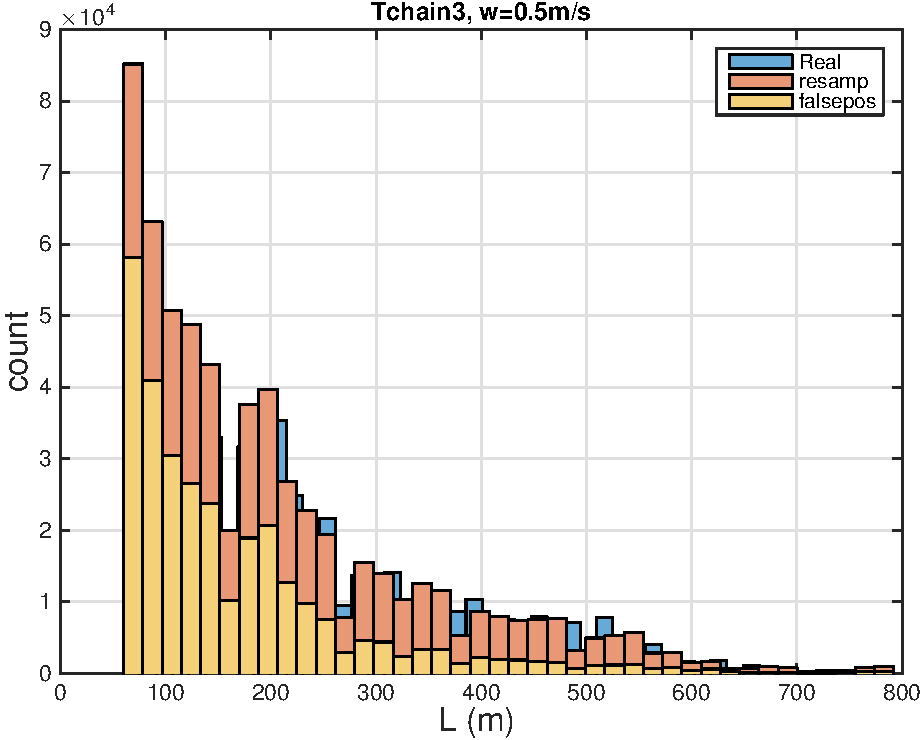
\includegraphics[scale=0.8]{Tchain3_Test2_LotHistFalsePos.pdf}
\caption{Histogram of overturn sizes for ensemble of resampled data at Tchain 3.  Three sets of data are plotted: (1) Real overturns (true overturns in Tchain data, but only at times corresponding to resampled profiles). (2) All overturns in resampled data. (3) False positive overturns: overturns in resampled data where true profile was stable.}
\label{T3_FalsePosHist}
\end{figure}


\begin{figure}[htbp]
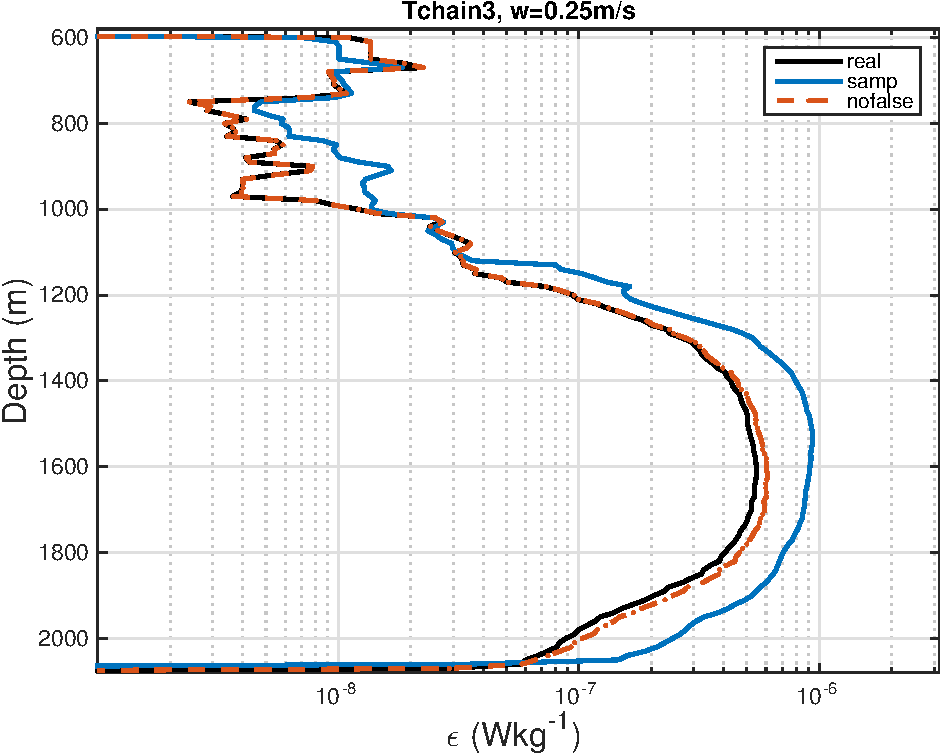
\includegraphics[scale=0.8]{Tchain3_Test1_EpsProfFalsePos.pdf}
\caption{ Time-mean profiles of epsilon from resampling at Tchain 3. Three sets of data are plotted: (1) `Real` (using  Tchain data, but only at times corresponding to resampled profiles). (2) All resampled profiles. (3) Resampled, but without false positive overturns (overturns in resampled data where true profile was stable).}
\label{T3_FalsePosProf}
\end{figure}


\begin{figure}[htbp]
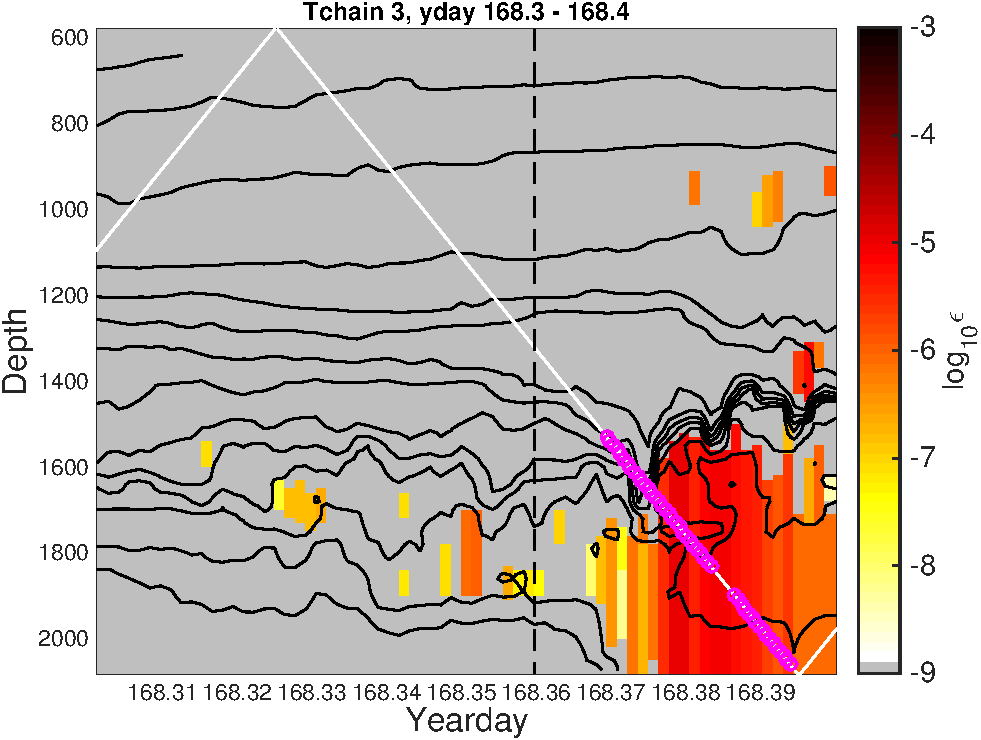
\includegraphics[scale=0.8]{Tchain3_Test1_ExampleFalsePos.pdf}
\caption{ Example of how false overturns could be introduced.}
\label{exampleFalsePos}
\end{figure}


\clearpage
%~~~~~~~~~~~~~~~~~
\subsection{28 Jan 2015}

\vskip
Wrote a code (\verb+CombineResampTestCases.m+) to put entire ensemble in one structure, along with the real profiles at matching times, so I don't have to write a loop for every analysis. 
\vskip
Found and finally fixed a problem finding and plotting false overturns introduced in the resampled data. I was using \verb+[R,C]=find(X)+ and then \verb+X(R,C)+ to plot, but this doesn't work like I thought it did. Just using single index now.
\vskip



%~~~~~~~~~~~~~~~~~
\subsection{27 Jan 2015}

I wanted to check the effect of using different minimum overturn sizes for the T-chains. The T-chain data is gridded to 10m, but the vertical spacing of the sensors was actually around 50m. According to Nyquist theorem, we should only be able to resolve overturns larger than 100m (with no noise). I thought the dissipation was probably dominated by the larger overturns, but wanted to check : \verb+CompareOverturnsDiffminOT.m+ .  At T-chain 3 the time-mean profile of epsilon is the same for minOT of 50m. For minOT of 100m, epsilon is smaller in the upper portion but the same in the region of largest dissipation below 1200m. At minOT of 250m, it has the same profile below 1200 but is smaller in magnitude. Results are similar at T-chain 4. This confirms that epsilon is dominated by larger overturns, except in the upper region.


Up to now I had assumed that the resampled overturn sizes were being symmetrically under/over estimated, leading to the increased average epsilon. Histograms of the difference in L are approximately normal and symmetric. However the story may be more complicated than this. I made scatter plots of the difference in L versus the true L (see \verb+ScatterErrorsVsTrue.m+), and there seems to be a negative trend. At lower true L, the differences are mostly positive (resampled L is larger than true L), while at larger true L, the differences are mostly negative. I would have expected the magnitude of the difference to depend on the true size, but I don't know why the sign would change. And smaller sampled L should make epsilon smaller, but the average epsilon is bigger.


I'm contouring epsilon and isotherms and plotting where false overturns are introduced in the resampled data, as well as where the resampled overturns are smaller or larger than the true size (\verb+ExamineShortSectionsResamp.m+). 






%
%

\end{document}  
